\chapter{Vector Bundles}\label{chapter:vector_bundles}

    The main reference for this chapter is~\citet{bott_differential_1995}.

    \minitoc

\section{Tangent bundle}

    The tangent space, as introduced in \cref{section:tangent_space}, can also be introduced in a more abstract and general way. Because it is the most important example of a vector bundle, tangent bundles are introduced first.

    \begin{construct}[Tangent bundle]\index{tangent!bundle}\label{bundle:tangent_bundle}
        Let $M$ be an $n$-dimensional manifold with atlas $\{(U_i,\varphi_i)\}_{i\leq n}$. Construct, for every open set $U$, an associated set $TU := U\times\mathbb{R}^n$ and construct, for every smooth function $f:U\rightarrow\mathbb{R}$, an associated smooth function on $TU$, called the \textbf{differential} or \textbf{derivative} of $f$, as follows:
        \begin{gather}
            \label{bundle:T_function}
            Tf:U\times\mathbb{R}^n\rightarrow f(U)\times\mathbb{R}^n:(p,v)\mapsto\bigl(f(p),Df(p)v\bigr)\,,
        \end{gather}
        where $Df(p):\mathbb{R}^n\rightarrow\mathbb{R}^n$ is the Jacobian of $f$ at $p$.

        By applying this definition to the transition functions $\psi_{ji}$, one obtains a new set of functions $T\psi_{ji}:TU_i\rightarrow TU_j$ given by
        \begin{gather}
            T\psi_{ji}(\varphi_i(p),v) := \left(\varphi_j(p),D(\varphi_j\circ\varphi_i^{-1})(\varphi_i(p))v\right)\,.
        \end{gather}
        Because the transition functions are diffeomorphisms, the associated Jacobians are invertible. This implies that the maps $T\psi_{ji}$ are represented by elements of $\GL(\mathbb{R}^n)$. The tangent bundle is then obtained by applying the Construction Theorem~\ref{bundle:fibre_bundle_construction_theorem} to the triple $(M,\mathbb{R}^n,\GL(\mathbb{R}^n))$ together with the cover $\{U_i\}_{i\leq n}$ and the cocycle $\{T\psi_{ji}\}_{i,j\leq n}$.
    \end{construct}

    \newdef{Natural chart}{\index{natural!chart}\index{adapted!chart|see{natural chart}}
        The charts in the atlas of this bundle are sometimes called natural charts or \textbf{adapted charts} because the first $n$ coordinates are equal to the coordinates on the base manifold.
    }

    \newdef{Tangent space}{\index{tangent!space}
        Consider a point $p\in M$. The definition of the tangent space in the bundle setting is given by the fibre
        \begin{gather}
            T_pM := \pi_{TM}^{-1}(p)\,.
        \end{gather}
        If one uses the natural charts identify $T_pM$ with the set $\varphi_i(p)\times\mathbb{R}^n$, it can be seen that $T_pM$ is isomorphic to $\mathbb{R}^n$ (as a vector space).
    }

    \begin{property}[Smooth structure]
        An atlas on $TM$ is given by the charts $(TU_i,\theta)$ with
        \begin{gather}
            \theta:TU_i\rightarrow\mathbb{R}^{2n}:(p,X)\mapsto(\varphi_i\circ\pi(p),X^1,\ldots,X^n)\,,
        \end{gather}
        where $(U_i,\varphi_i)$ is a chart around $p\in M$ such that a tangent vector $X$ is trivialized as $X^i\partial_i\in T_pM$.
    \end{property}

    \begin{property}[Dimension]
        Let $M$ be an $n$-dimensional manifold. Using the charts on $M$ and the adapted charts on $TM$, one can see that $TM$ is locally isomorphic to $\mathbb{R}^{2n}$. This implies that
        \begin{gather}
            \dim(TM) = 2\dim(M)\,.
        \end{gather}
    \end{property}

    \begin{remark}[Physics]
        Now, it should be clear that the statement ``\textit{a vector is something that transforms like a vector}'', which one often hears in introductory physics courses, comes from the fact that \[\text{a vector }v\in T_pM\text{ is tangent to }\varphi_i(p)\text{ in a chart }(U_i,\varphi_i)\] if and only if \[D(\varphi_j\circ\varphi_i^{-1})(\varphi_i(p))v\text{ is tangent to }\varphi_j(p)\text{ in a chart }(U_j,\varphi_j)\,.\]
    \end{remark}

    \newdef{Differential}{\index{differential}\label{bundle:differential}
        The map $T$ defined in \cref{bundle:T_function} can be generalized to arbitrary smooth manifolds as the map $Tf:TM\rightarrow TN$, which is locally represented by the Jacobian. Furthermore, let $p\in U\subseteq M$ and let $V = f(U)$. By looking at the restriction of $Tf$ to $T_pM$, one can see that it maps $T_pU$ to $T_{f(p)}V$ linearly.
    }

    \begin{property}\index{derivative!functorial}
        The map $Tf:TM\rightarrow TN$ has the following properties:
        \begin{itemize}
            \item $T$ preserves identities: $T\mathbbm{1}_M = \mathbbm{1}_{TM}$.
            \item Let $f,g$ be two smooth functions on smooth manifolds, then $T(f\circ g) = Tf\circ Tg$.
        \end{itemize}
        This turns the map $T$ into an endofunctor (\cref{cat:endofunctor}) on the category of smooth manifolds. One can view $T$ as a `functorial derivative'.
    \end{property}

    \newdef{Rank}{\index{rank!of a function}\label{bundle:rank}
        Let $f:M\rightarrow N$ be a differentiable function between smooth manifolds. Using the fact that $Tf$ is fibrewise linear, the rank of $f$ at $p\in M$ is defined as the rank of the differential $Tf:T_pM\rightarrow T_{f(p)}N$ in the sense of \cref{linalgebra:image_rank}.
    }

    \begin{theorem}[Inverse function theorem]\index{inverse function theorem}\index{local!diffeomorphism}\label{bundle:inverse_function_theorem}
        A smooth function $f:M\rightarrow N$ between smooth manifolds is a local diffeomorphism at $p\in M$ if and only if its differential $Tf:T_pM\rightarrow T_{f(p)}N$ is an isomorphism at $p$.
    \end{theorem}

    \newdef{Parallelizable manifold}{\index{parallelizable}
        A manifold with a trivial tangent bundle.
    }

\section{Vector bundles}

    Instead of restricting the typical fibre to be a Euclidean space with the same dimension as the base manifold, one can generalize the construction of the tangent bundle in the following way.
    \begin{construct}[Vector bundle]\index{vector!bundle}\index{rank!of a vector bundle}\label{bundle:vector_bundle_construction}
        Consider a (topological) manifold with an atlas $\{(U_i,\varphi_i)\}_{i\in I}$, a cocycle $\{g_{ji}:U_i\cap U_j\rightarrow G\}_{i,j\in I}$ with values in a group $G$ and a representation $\rho:G\rightarrow\GL(V)$ on a (finite-dimensional) vector space $V$. This data can be used to construct a fibre bundle through \cref{bundle:fibre_bundle_construction_theorem}. The dimension of the typical fibre $V$ is called the \textbf{rank} of the vector bundle.
    \end{construct}
    \begin{remark}
        As was also the case for tangent bundles, the choice of charts on $E$ is not random. To preserve the linear structure of fibres, the use of the natural charts is imperative.
    \end{remark}

    \begin{example}[Line bundle]\index{line!bundle}\index{wave!function}
        A vector bundle with a one-dimensional fibre. A common example in quantum mechanics is the $\mathbb{C}$-line bundle over some smooth manifold whose sections correspond to the \textit{wave functions} of a given system. (See \cref{section:geometric_quantization} on geometric quantization for more information.)
    \end{example}

    \begin{property}[Vector bundles over a sphere]\label{bundle:vector_bundles_over_sphere}
        The Clutching Theorem~\ref{bundle:clutching_theorem} and the homotopy invariance imply that rank-$p$ vector bundles over the sphere are determined by homotopy classes of functions $S^{n-1}\rightarrow\GL_p(\mathfrak{K})$, i.e.~they are classified by the homotopy group $\pi_{n-1}(\GL_p(\mathfrak{K}))$.
    \end{property}

\subsection{Sections}

    \newdef{Frame}{\index{frame}\label{bundle:frame}
        A frame of a vector bundle $E$ is a tuple $(s_1,\ldots,s_n)$ of sections such that $(s_1(b),\ldots,s_n(b))$ is a basis for the fibre $\pi^{-1}(b)$ for all $b\in B$. By passing to local sections, one obtains a local frame.
    }
    \begin{property}[Trivial bundles]\label{bundle:trivial_vector_bundle}
        A vector bundle is trivial if and only if it admits a global frame.
    \end{property}

    \begin{theorem}[Serre \& Swan]\index{Serre--Swan}\label{bundle:serre_swan}
        The set of smooth sections of a smooth vector bundle over a smooth manifold $M$ is a finitely generated projective $C^\infty(M)$-module. More generally, the set of sections of a vector bundle over a compact Hausdorff manifold $B$ is a finitely generated projective $C(B)$-module.
    \end{theorem}

    \newdef{Zero section}{\label{bundle:zero_section}
        The section $s_0$ of a vector bundle $E\rightarrow B$ that assigns to every point $b\in B$ the zero vector of the associated fibre $E_b$. For every vector bundle $\pi:E\rightarrow B$, one can embed the base manifold $B$ in the bundle $E$ through the zero section $s_0:B\rightarrow E$. The complement of the image of this section is often denoted by $E_0$.
    }

\subsection{Tubular neighbourhoods}

    \newdef{Normal bundle}{\index{normal!bundle}
        Consider a smooth manifold $M$ with a submanifold $S$ and consider, for every point $p\in S$, the tangent spaces $T_pS$ and $T_pM$. Since $T_pS$ is a subspace of $T_pM$, one can construct the quotient space $N_pS := T_pM/T_pS$. The normal bundle of $S$ in $M$ is defined as the vector bundle with fibres $N_pS$.
    }
    \newdef{Tubular neighbourhood}{\index{tubular neighbourhood}\label{bundle:tubular_neighbourhood}
        Consider a smooth manifold $M$ with an embedded submanifold $S$. A tubular neighbourhood of $S$ in $M$ is a vector bundle $\pi:E\rightarrow S$ such that (an open neighbourhood of the zero section of) $E$ is diffeomorphic to an open neighbourhood of $S$ in $M$.
    }
    \begin{theorem}[Tubular neighbourhood theorem]\label{bundle:tubular_neighbourhood_theorem}
        Every embedded submanifold admits a tubular neighbourhood, namely its normal bundle. Furthermore, all tubular neighbourhoods are diffeomorphic.
    \end{theorem}
    \begin{result}[NDR pairs]\label{bundle:ndr_submanifold}
        Consider a smooth manifold $M$ with a submanifold $S$. The pair $(M,S)$ is an NDR pair (\cref{topology:ndr_pair_homology}). In particular, consider a smooth fibre bundle $\pi:E\rightarrow B$. If $\pi$ admits a global section, one can embed $B$ in $E$ as a submanifold and, hence, the pair $(E,B)$ is an NDR pair.
    \end{result}

\subsection{Sums and product}

    \newdef{Whitney sum}{\index{Whitney!sum}\index{direct!sum}
        Consider two vector bundles $E,E'$ with typical fibres $V,V'$ over the same base space. One can construct a new vector bundle $E\oplus E'$ by taking the typical fibre to be the direct sum $V\oplus V'$, i.e.~the fibre over $p$ is given by $V_p\oplus V_p'$. This operation is called the Whitney sum or \textbf{direct sum} of vector bundles.
    }

    The existence property for complements (\cref{linalgebra:complement}) from linear algebra can be generalized in the following way.
    \begin{property}
        Let $B$ be a paracompact Hausdorff manifold and let $E$ be a vector bundle over $B$. Every vector subbundle $F$ of $E$ admits an orthogonal complement $F^\perp$.
    \end{property}
    \begin{property}\label{bundle:hausdorff}
        Let $B$ be a compact Hausdorff manifold. Every vector bundle $E$ over $B$ admits a complementary vector bundle $E^c$ such that $E\oplus E^c\cong B\times\mathbb{R}^n$ for some $n\in\mathbb{N}$.
    \end{property}

    \newdef{Stable isomorphism}{\index{stable!isomorphism}\label{bundle:stable_isomorphism}
        Two vector bundles $E,E'$ over a base space $B$ are said to be stably isomorphic if there exist integers $m,n\in\mathbb{N}$ such that
        \begin{gather}
            E\oplus(B\times\mathbb{R}^m)\cong E'\oplus(B\times\mathbb{R}^n)\,.
        \end{gather}
    }

    \newdef{Tensor product}{\index{tensor product!of vector bundles}
        The tensor product $E\otimes E'\rightarrow B$ of two vector bundles $\pi:E\rightarrow B$ and $\pi':E'\rightarrow B$ is given by the fibrewise tensor product.
    }
    \newdef{Exterior tensor product}{\index{tensor product!exterior}
        The exterior tensor product $E\boxtimes E'\rightarrow B\times B'$ of two vector bundles $\pi:E\rightarrow B$ and $\pi':E'\rightarrow B'$ is given by the tensor product of fibres over the Cartesian product $B\times B'$.
    }

\subsection{Associated vector bundles}

    \begin{construct}[Associated vector bundle]\index{associated!vector bundle}\label{bundle:associated_vector_bundle}
        Consider a representation \[\rho:\GL(\mathbb{R}^n)\rightarrow\GL(\mathbb{R}^l)\] together with the tangent bundle cocycle $\{t_{ji} := D(\psi_{ji})\circ\varphi_i\}_{i,j\leq n}$. The composite \[\rho\circ t_{ji}:U_i\cap U_j\overset{t_{ji}}{\rightarrow}\GL(\mathbb{R}^n)\overset{\rho}{\rightarrow}\GL(\mathbb{R}^l)\] is again a cocycle and can be used to define a new vector bundle on $M$ through the fibre bundle construction theorem. The vector bundle $\rho(TM)$ is called the associated (vector) bundle of the tangent bundle induced by $\rho$.
    \end{construct}

    \begin{example}[Contravariant vectors]\index{contra-!variant}
        By noting that the $k^{\text{th}}$ tensor power $\otimes^k$ induces a representation given by the tensor product of representations, one can construct the bundle of order-$k$ (contravariant) tensors $\otimes^k(TM)$.
    \end{example}
    \begin{example}[Cotangent bundle]\index{covariant}\index{co-!vector}\label{bundle:cotangent_bundle}
        Another useful construction is given by the contragredient representation $(\rho^T)^{-1}=(\rho^{-1})^T$. The vector bundle constructed this way, where the cocycle is given by $(t_{ji}^T)^{-1}$, is called the cotangent bundle on $M$ and is denoted by $T^*M$. Elements of the fibres are called \textbf{covariant vectors} or \textbf{covectors}.
    \end{example}
    \begin{notation}
        A combination of the cocycle $t_{ji}$ and its dual $(t_{ji}^T)^{-1}$ can also be used to define the bundle of $(k,l)$-tensors on $M$. This bundle is denoted by $T^{(k,l)}M$.
    \end{notation}

    \newdef{Twisted bundle}{\index{twist}
        Given a vector bundle $\pi:E\rightarrow B$ and a line bundle $\psi:L\rightarrow B$, one calls the tensor product $E\otimes L$ the $L$-twisted version of $E$.
    }

    For every vector bundle, one can define a canonical line bundle.
    \begin{construct}[Determinant line bundle]\index{bundle!determinant}\index{determinant!line bundle|see{bundle, determinant}}\index{density}
        Consider a rank-$n$ vector bundle $\pi:E\rightarrow B$. The determinant map induces an associated line bundle $\det(\pi):\bigwedge^nE\rightarrow B$, where the transition functions on the fibres are given by the determinant of the transition functions of $E$. Bundles twisted by a determinant line bundle $\det(E)$ are called \textbf{densitized bundles}.\footnote{See also \cref{bundle:honest_density}.}
    \end{construct}
    \begin{example}[Canonical bundle]\index{bundle!canonical}\label{bundle:canonical_bundle}
        Consider a smooth manifold $M$. The canonical (line) bundle of $M$ is given by $\det(T^*M)=\Omega^{\dim(M)}(M)$, the determinant line bundle of the cotangent bundle of $M$.
    \end{example}

\section{Vector fields}

    From here on, the theory will be specialized to the smooth setting, i.e.~all manifolds and all morphisms will be assumed to be smooth (unless stated otherwise).

    \newdef{Vector field}{\index{vector field}
        A section $s\in\Gamma(TM)$ of the tangent bundle. By the Serre--Swan theorem~\ref{bundle:serre_swan}, the set of vector fields forms a $C^\infty(M)$-module.
    }
    \begin{notation}
        The set of all vector fields on a manifold $M$ is often denoted by $\mathfrak{X}(M)$.
    \end{notation}

    \newdef{Index}{\index{index}
        Consider a vector field $X$ on an $n$-dimensional manifold $M$ and let $p\in M$ be an isolated zero of $X$. Because $p$ is isolated, one can find a small $(n-1)$-sphere around $p$ that does not contain any other zeroes of $X$. The index $\text{ind}_X(p)$ of $X$ at $p$ is defined as the degree (\cref{topology:degree}) of the function
        \begin{gather}
            f:S^{n-1}\rightarrow S^{n-1}:m\mapsto\frac{X(m)}{\|X(m)\|}\,.
        \end{gather}
    }
    \begin{property}[Winding number]\index{winding number}
        The winding number of a vector field $X$ along a curve $\gamma$ on which $X$ does not vanish is equal to the sum of indices of zeroes of $X$ lying inside $\gamma$.
    \end{property}

    \begin{theorem}[Poincar\'e--Hopf]\index{Poincar\'e--Hopf}\index{Euler!characteristic}\label{bundle:poincare_hopf}
        Let $M$ be a compact manifold and consider a vector field $X$ having only isolated zeroes. The Euler characteristic (\cref{topology:euler_characteristic}) is given by
        \begin{gather}
            \chi(M)=\sum_{p\in X^{-1}(0)}\mathrm{ind}_X(p)\,.
        \end{gather}
    \end{theorem}
    \begin{remark}
        This is essentially a restatement of \cref{manifold:euler_characteristic}, where one submanifold is given by the zero section and the other is given by the graph of $X$.
    \end{remark}

    An immediate consequence of the Poincar\'e--Hopf theorem is the following well-known result.
    \begin{theorem}[Hairy ball theorem]\index{hairy ball theorem}
        There exists no nowhere-vanishing vector field on an even-dimensional sphere $S^{2n}$.
    \end{theorem}

    \newdef{Pullback}{\index{pullback!of a vector field}\label{bundle:pullback}
        Consider a diffeomorphism $\varphi:M\rightarrow N$ and let $X$ be a vector field on $N$. The pullback of $X$ along $\varphi$ is defined as follows:
        \begin{gather}
            (\varphi^*X)_p := T\varphi^{-1}(X_{\varphi(p)})\,.
        \end{gather}
    }
    \newdef{Pushforward}{\index{pushforward!of a vector field}\label{bundle:pushforward}
        Let $X$ be a vector field on $M$ and let $\varphi:M\rightarrow N$ be a diffeomorphism. The pushforward of $X$ along $\varphi$ is defined as follows:
        \begin{gather}
            (\varphi_*X)_{\varphi(p)} := T\varphi(X_p)\,.
        \end{gather}
        This can be rewritten using the pullback as follows:
        \begin{gather}
            \label{bundle:pullback_pushforward}
            \varphi_*X = (\varphi^{-1})^*X\,.
        \end{gather}
        Equivalently, one can define a vector field on $N$ as
        \begin{gather}
            (\varphi_*X)_q(f) := X_{\varphi^{-1}(q)}(f\circ\varphi)\,.
        \end{gather}
    }

    \begin{example}[Projective space]\index{Euler!operator}\label{bundle:projective_space}
        Consider the manifold $\mathbb{CP}^n$ for some $n\in\mathbb{N}$. Local coordinate patches are given by charts
        \begin{gather}
            \mathbb{C}^n\rightarrow \pi_i:U_i:(x_1,\ldots,x_n)\mapsto\left[x_1:\ldots:x_i:1:x_{i+1}:\ldots:x_n\right]\,,
        \end{gather}
        where $U_i:=\{[x]\in\mathbb{CP}^n\mid x\in\mathbb{C}^{n+1},x_i\neq0\}.$ To determine the vector fields induced by the basis vector fields $\partial_i$, however, it is more useful to start from the quotient map $\pi:\mathbb{C}^{n+1}/\{0\}\rightarrow\mathbb{CP}^n$. This map acts on the subset $\{x\in\mathbb{C}^{n+1}\mid x_i\neq 0\}$ as
        \begin{gather}
            (x_1,\ldots,x_{n+1})\mapsto\left[\frac{x_1}{x_i}:\cdots:\frac{x_{i-1}}{x_i}:1:\frac{x_{i+1}}{x_i}:\cdots:\frac{x_{n+1}}{x_i}\right]
        \end{gather}
        to give the chart $U_i$. Locally on this subset, pushing the $n+1$ basis vector fields $\partial_i$ forward along $\pi$ gives
        \begin{gather}
            \begin{cases}
                \ds\pi_\ast\partial_j = \frac{1}{x_i}\widetilde\partial_j&\cif j\neq i\,,\\&\\
                \ds\pi_\ast\partial_i = -\sum_{j\neq i}\frac{x_j}{x_i^2}\widetilde\partial_j&\text{otherwise}\,.
            \end{cases}
        \end{gather}
        The kernel of this projection is given by the Euler vector field
        \begin{gather}
            \mathbb{E} := x^i\partial_i
        \end{gather}
        from \cref{calculus:euler_operator}.
    \end{example}

\subsection{Integral curves}

    \newdef{Integral curve}{\index{integral!curve}\label{bundle:integral_curve}
        Let $X\in\mathfrak{X}(M)$ and let $\gamma:\ ]a,b[\ \rightarrow M$ be a curve on $M$. $\gamma$ is called an integral curve of $X$ if
        \begin{gather}
            \gamma'(t) = X(\gamma(t))
        \end{gather}
        for all $t\in\ ]a,b[$\,, where $\gamma'(t) := T\gamma(t,1)$.

        This equation can be viewed as a system of ordinary differential equations. Using the Picard--Lindel\"of existence theorem~\ref{ode:picard_lindelof}, together with the initial value condition $\gamma(0)=p$, one can find a unique maximal curve satisfying the above equation. This solution, denoted by $\gamma_p$, is called the \textbf{integral curve of $X$ through $p$}.
    }

    \newdef{Flow}{\index{flow}\label{bundle:flow}
        Let $X\in\mathfrak{X}(M)$ and consider its integral curve $\gamma_p$ through a point $p\in M$. The function $\sigma_t$ defined by
        \begin{gather}
            \sigma_t(p) := \gamma_p(t)\,,
        \end{gather}
        is called the flow of $X$ at time $t$. The \textbf{flow domain} is defined as the set
        \begin{gather}
            D(X) := \bigl\{(t,p)\in\mathbb{R}\times M\bigm\vert p\in M,t\in\ ]a_p,b_p[,a_p<0<b_p\bigr\}\,,
        \end{gather}
        where $]a_p,b_p[$ is the maximal interval on which $\gamma_p$ is defined.
    }
    \begin{property}
        Suppose that $D(X) = \mathbb{R}\times M$. The flow $\sigma_t$ has the following properties for all $s,t\in\mathbb{R}$:
        \begin{itemize}
            \item $\sigma_t$ is smooth,
            \item $\sigma_0 = \mathbbm{1}_M$,
            \item $\sigma_{s+t} = \sigma_s\circ\sigma_t$, and as a consequence
            \item $\sigma_{-t} = (\sigma_t)^{-1}$.
        \end{itemize}
        These properties say that $\sigma_t$ is a diffeomorphic group action of the additive group of real numbers on $M$. This implies that $\sigma_t$ is a (smooth) flow in the general mathematical sense.
    \end{property}

    \newdef{Complete vector field}{\index{complete!vector field}\label{bundle:complete_vector_field}
        A vector field on a manifold $M$ for which the flow domain for every flow is all of $\mathbb{R}\times M$.
    }

    \begin{property}
        If the manifold $M$ is compact, every vector field $X\in\mathfrak{X}(M)$ is complete.
    \end{property}

    \begin{property}[Winding number]\index{winding number}
        The winding number of a vector field along a closed integral curve is 1.
    \end{property}

\subsection{Lie derivative}

    \newdef{Lie derivative for smooth functions}{\index{Lie!derivative}\label{bundle:lie_derivative_functions}
        Consider $X\in\mathfrak{X}(M)$ and $f\in C^\infty(M)$. The Lie derivative of $f$ with respect to $X$ at $p\in M$ is defined as
        \begin{gather}
            \mathcal{L}_Xf(p) := \lim_{t\rightarrow0}\frac{f\bigl(\gamma_p(t)\bigr) - f(p)}{t}\,.
        \end{gather}
    }
    The definition of the Lie derivative closely resembles the definition of the ordinary derivative on Euclidean space. This is not a coincidence.
    \begin{formula}\label{bundle:lie_derivative_function}
        Working out the definition of the Lie derivative and rewriting it as an operator equality gives
        \begin{gather}
            \label{bundle:lie_derivative_function_expansion}
            \mathcal{L}_X = \sum_kX^k\pderiv{}{x^k}\,.
        \end{gather}
        It is clear that this is just the vector field $X$ expressed in the basis of \cref{manifold:tangent_vector_partial}. This way, one also recovers the behaviour of a tangent vector as a derivation. For smooth functions $f:M\rightarrow\mathbb{R}$, this gives
        \begin{gather}
            \mathcal{L}_Xf(p) = X_p(f)\,.
        \end{gather}

        \begin{mdframed}[roundcorner=10pt, linecolor=blue, linewidth=1pt]
            \begin{proof}[Explanation]
                In this derivation, Landau's little-o notation is used:
                \begin{gather}
                    \lim_{t\rightarrow0}\frac{o(t)}{t} = 0.
                \end{gather}
                Now, assume that $X$ is a smooth vector field and $f$ is a smooth function. Because the Lie derivative is a local operation one can work in a local chart such that $\gamma$ is, again locally, equivalent to a curve\footnote{The vector field $X(p) = (p,Y(p))$, where $Y$ is a smooth vector field on $\mathbb{R}^n$, can also be identified with $Y$ itself. This is implicitly done in the derivation by using the notation $X$ for both vector fields.} $\beta_p:U\rightarrow\mathbb{R}^n$ and such that one can expand $\beta_p(t)$ around $p\in U$:
                \begin{align}
                    \mathcal{L}_Xf(p) &= \lim_{t\rightarrow0}\left[\frac{f(\beta_p(0) + t\beta_p'(0) + o(t)) - f(p)}{t}\right]\nonumber\\
                    &= \lim_{t\rightarrow0}\left[\frac{f(p + tX(p) + o(t)) - f(p)}{t}\right]\nonumber\\
                    &= \lim_{t\rightarrow0}\left[\frac{f(p) + tDf(p)\cdot X(p) + o(t) - f(p)}{t}\right]\nonumber\\
                    &= \sum_k\pderiv{f}{x^k}(p)X_k(p) + \lim_{t\rightarrow0}\frac{o(t)}{t}\nonumber\\
                    &= \sum_k\pderiv{f}{x^k}(p)X_k(p)\,,\label{diff:lie_derivative_calc}
                \end{align}
                where \cref{bundle:integral_curve} for integral curves was used on the second line. If this equation is rewritten as an operator equality, one obtains
                \begin{gather}
                    \mathcal{L}_X = \sum_kX_k\pderiv{}{x^k}\,.
                \end{gather}$ $
            \end{proof}
        \end{mdframed}
    \end{formula}

    \newdef{Lie derivative for vector fields}{\label{bundle:lie_derivative_vector_field}
        Let $X,Y\in\mathfrak{X}(M)$.
        \begin{gather}
            \mathcal{L}_XY(p) := \left.\deriv{}{t}(\sigma_t^*X)(\gamma_p(t))\right|_{t=0}\,.
        \end{gather}
        \begin{mdframed}[roundcorner=10pt, linecolor=blue, linewidth=1pt]
            \begin{proof}[Explanation]
                For vector fields one cannot just take the difference at two different points because the tangent spaces generally do not coincide. This can be resolved by using the flow (\cref{bundle:flow}):
                \begin{gather}
                    \label{derivmath:lie_derivative_vector_fields}
                    \mathcal{L}_XY = \lim_{t\rightarrow0}\frac{(T\sigma_t)^{-1}X(\gamma_p(t)) - X(p)}{t}\,,
                \end{gather}
                where $T\sigma_t$ is the differential (\cref{bundle:differential}) of the flow, which satisfies $(T\sigma)^{-1} = T\sigma_{-t}$. To see that this definition makes sense, one has to show that $(T\sigma_t)^{-1}[X(\gamma_p(t))]\in T_pM$. This goes as follows:
                \begin{align*}
                    (T\sigma_t)^{-1}X(\gamma_p(t))(f) &= T\sigma_{-t}X(\gamma_p(t))(f)\\
                    &= X(\sigma_{-t}\circ\gamma_p(t))(f\circ\sigma_{-t})\\
                    &= X(\sigma_{-t}\circ\sigma_t(p))(f\circ\sigma_{-t})\\
                    &= X(p)(f\circ\sigma_{-t})\\
                    &\in T_pM
                \end{align*}
                for all $f\in C^k(M,\mathbb{R})$. On the third line, the definition of the flow was used. One can also rewrite the second term in the numerator of \cref{derivmath:lie_derivative_vector_fields} using the flow: \[X(p) = X(\sigma_0(p)) = T\sigma_0(X)\,.\] Using the definition of the pushforward of vector fields (\cref{bundle:pushforward}), the Lie derivative can be rewritten as follows:
                \begin{align*}
                    \mathcal{L}_XY &= \lim_{t\rightarrow0}\frac{\sigma_{-t*}X(\gamma_p(t)) - \sigma_{0*}X(\gamma_p(0))}{t}\\
                    &= \left.\deriv{}{t}(\sigma_{-t*}X)(\gamma_p(t))\right|_{t=0}\,.
                \end{align*}
                Finally, by using the relation~\eqref{bundle:pullback_pushforward} between pushforward and pullback, this becomes
                \begin{gather}
                    \mathcal{L}_XY = \left.\deriv{}{t}(\sigma_t^*X)(\gamma_p(t))\right|_{t=0}\,.
                \end{gather}$ $
            \end{proof}
        \end{mdframed}
    }
    \begin{property}[Lie bracket]\index{Lie!bracket}\label{bundle:lie_bracket}
        Let $X,Y\in\mathfrak{X}(M)$ be $C^k$-vector fields. The Lie derivative has the following properties:
        \begin{itemize}
            \item $\mathcal{L}_XY$ is a vector field.
            \item The Lie derivative of vector fields coincides with the commutator:
                \begin{gather}
                    \mathcal{L}_XY = [X,Y]\,.
                \end{gather}
                The fact that this is indeed a derivation on $C^{k-1}(M,\mathbb{R})$ follows from Schwarz's theorem~\ref{calculus:schwarz_theorem}. This result shows that the Lie derivative on vector fields turns the space $\mathfrak{X}(M)$ into a (real) Lie algebra.
            \item The previous item also implies that the Lie derivative is antisymmetric:
                \begin{gather}
                    \label{bundle:lie_derivative_antisymmetry}
                    \mathcal{L}_XY = -\mathcal{L}_YX\,.
                \end{gather}
        \end{itemize}
    \end{property}

    \newdef{Holonomic basis}{\index{holonomic!basis}
        Consider a smooth manifold $M$ and an open subset $U\subseteq M$. A local frame $\{e_i\}_{i\leq\dim(M)}$ for $TU$ is said to be holonomic if all the Lie derivatives vanish on $U$:
        \begin{gather}
            \mathcal{L}_{e_i}e_j = 0\,.
        \end{gather}
        Equivalently, a basis is holonomic if the associated structure coefficients of the Lie algebra $\mathfrak{X}(M)$ vanish on $U$.
    }
    \begin{property}
        For every holonomic basis, there exists a coordinate system on $M$ such that the basis coincides with the coordinate-induced basis.
    \end{property}

\subsection{Multivector fields}

    Similar to the construction of \textit{differential forms} in \cref{section:forms} below, one can also construct products of vector fields.

    \newdef{Multivector field}{
        A section of the exterior algebra $\Lambda^\bullet TM$.
    }

    \newdef{Schouten--Nijenhuis bracket}{\index{Schouten--Nijenhuis bracket}\label{bundle:schouten_nijenhuis_bracket}
        The unique extension of the Lie bracket to multivector fields that turns $\Gamma(\Lambda^\bullet TM)$ into a Gerstenhaber algebra (\cref{hda:gerstenhaber_algebra}).

        A more explicit description is given as follows. Let $f\in C^\infty(M)$ and $\{X_i\}_{i\leq n}\in\mathfrak{X}(M)$ for some $n\in\mathbb{N}$.
        \begin{gather}
            [f,X_1\wedge\cdots\wedge X_n] := -\iota_{\dr f}X_1\wedge\cdots X_n\,,
        \end{gather}
        where $\dr f$ is the \textit{exterior derivative} (see \cref{bundle:exterior_derivative}) and $\iota$ is defined analogous to \cref{bundle:interior_derivative},
        and
        \begin{gather}
            [X_1\wedge\cdots\wedge X_{i_k}, X_{i_{k+1}}\wedge\cdots\wedge X_n] := \sum_{i,j}[X_i,X_j]X_1\wedge\cdots\wedge\hat{X}_i\wedge\cdots\wedge\hat{X}_j\wedge\cdots\wedge X_n
        \end{gather}
        for all $k\leq n$, where the caret indicates that this vector field is omitted. The Schouten--Nijenhuis bracket of two smooth functions is defined to be identically zero.
    }

\section{Differential \texorpdfstring{$k$}{k}-forms}\label{section:forms}
\subsection{Definition}

    \newdef{Differential form}{\index{differential form}
        A differential $k$-form is a map
        \begin{gather}
            \omega:T^kM\rightarrow\mathbb{R}
        \end{gather}
        such that the restriction of $\omega$ to each fibre of the bundle $T^kM$ is multilinear and antisymmetric. The space of all differential $k$-forms on a manifold $M$ is denoted by $\Omega^k(M)$. Just like $\mathfrak{X}(M)$, it forms a $C^\infty(M)$-module.
    }
    Differential forms can also be constructed as sections of an associated vector bundle.
    \begin{adefinition}
        Consider the representation \[\rho_k:\GL(\mathbb{R}^{m*})\rightarrow\GL(\Lambda^k\mathbb{R}^{m*}): A\mapsto A\wedge\cdots\wedge A.\] This representation induces an associated vector bundle $\rho_k(\pi_{T^*M})$ of the cotangent bundle on $M$. A differential $k$-form is given by a section of $\rho_k(\pi_{T^*M})$:
        \begin{gather}
            \Omega^k(M) := \Gamma(\rho_k(\pi_{T^*M}))\,.
        \end{gather}
    \end{adefinition}

    \begin{construct}[Exterior algebra]
        One can construct a Grassmann algebra (\cref{vector:exterior_algebra}) by equipping the graded vector space
        \begin{gather}
            \Omega^\bullet(M) := \bigoplus_{k\geq0}\Omega^k(M)
        \end{gather}
        with the wedge product of differential forms that is induced by the wedge product on $\Lambda^k\mathbb{R}^m$. This graded algebra is associative, graded-commutative and unital with the constant function $1\in C^{\infty}(M)$ as the identity element.
    \end{construct}

    \newdef{Pullback}{\index{pullback!of a differential form}\label{bundle:forms_pullback}
        Let $f:M\rightarrow N$ be a smooth function between manifolds and let $\omega$ be a differential $k$-form on $N$. The pullback of $\omega$ by $f$ is defined as
        \begin{gather}
            f^*\omega := \omega\circ f_*\,.
        \end{gather}
        This defines a map $f^*:\Omega^\bullet(N)\rightarrow\Omega^\bullet(M)$.
    }
    \newdef{Pushforward}{\index{pushforward!of a differential form}\label{bundle:forms_pushforward}
        Let $f:M\rightarrow N$ be a diffeomorphism between manifolds and let $\omega$ be a differential $k$-form on $M$. The pushforward of $\omega$ by $f$ is defined as
        \begin{gather}
            f_*\omega := \omega\circ(f^{-1})_*\,.
        \end{gather}
    }
    \begin{remark*}
        Note that the pushforward of differential $k$-forms is only defined for diffeomorphisms, in contrast to pullbacks which only require smooth functions. This also explains why differential forms are the most valuable elements in differential geometry. (Vector fields cannot even be pulled back by general smooth maps.)
    \end{remark*}

    \newformula{Dual basis}{\label{bundle:dual_basis}
        Consider the coordinate basis from \cref{manifold:tangent_vector_partial} for the tangent space $T_pM$. From this set, one can construct a natural dual basis for the cotangent space $T_p^*M$ using the natural pairing:
        \begin{gather}
            \left\langle\pderiv{}{x^i},\drx^j\right\rangle = \delta_i^j\,.
        \end{gather}
        It should be noted that $\drx^i$ is not just a notation. In the next section, it will be shown that these basis vectors can be obtained by applying the \textit{exterior derivative} to the coordinate functions $x^i$.
    }

\subsection{Exterior derivative}

    \newdef{Exterior derivative}{\index{exterior!derivative}\index{differential}\label{bundle:exterior_derivative}
        The exterior derivative $\dr_k$ is a morphism constructed on the graded algebra of differential $k$-forms:
        \begin{gather}
            \dr_k:\Omega^k(M)\rightarrow\Omega^{k+1}(M)\,.
        \end{gather}
        For $k=0$, it is defined by
        \begin{gather}
            \label{bundle:function_derivative}
            \dr f := \sum_{i=1}^n\pderiv{f}{x_i}\drx_i
        \end{gather}
        The object $\dr f\in\Omega^1(M)$ is often called the \textbf{differential} of $f$. This formula can be generalized to higher degree forms as follows:
        \begin{gather}
            \dr(f\drx_{i_1}\wedge\cdots\wedge\drx_{i_k}) := \dr f\wedge \drx_{i_1}\wedge\cdots\wedge\drx_{i_k}\,.
        \end{gather}
    }
    \remark{\Cref{bundle:function_derivative} should be compared with the (informal) formula for the differential of a function that is often used in physics. The main difference is that, here, the quantities $\drx^i$ are not infinitesimal quantities but vectors of unit norm.}

    \begin{property}\index{Leibniz!rule}\label{bundle:exterior_derivative_properties}
        The exterior derivatives satisfy the following properties for all $k\in\mathbb{N}$:
        \begin{itemize}
            \item\textbf{Nilpotency}: For all $\omega\in\Omega^k(M)$:
                \begin{gather}
                    \dr_k\circ\dr_{k+1} = 0\,.
                \end{gather}
            \item\textbf{Linearity}: $\dr_k$ is $\mathbb{R}$-linear.
        \end{itemize}
        These two items say that $(\Omega^\bullet(M),\dr)$ is not just a graded algebra, but in fact a dg-algebra (\cref{homalg:dg_algebra}).
        \begin{itemize}
            \item\textbf{Graded Leibniz rule}: (hence $\dr$ is a graded derivation):
                \begin{gather}
                    \dr(\omega_1\wedge\omega_2) = \dr\omega_1\wedge\omega_2 + (-1)^j\omega_1\wedge\dr\omega_2\,,
                \end{gather}
                where $\omega_1\in\Omega^j(M)$ and $\omega_2\in\Omega^k(M)$.
            \item\textbf{Naturality}: If $f\in C^\infty(M)$, then $f^*(\dr\omega) = \dr(f^*\omega)$.
        \end{itemize}
    \end{property}

    \begin{formula}
        Let $f\in C^\infty(M,\mathbb{R})$ and let $\gamma$ be a curve on $M$. From \cref{bundle:dual_basis} of the basis $\{\drx_k\}_{k\leq n}$, one obtains the following result:
        \begin{gather}
            \langle\dr f(x),\gamma'(t)\rangle = \sum_k\pderiv{f}{x_k}(x)\gamma_k'(t) = (f\circ\gamma')(t)\,.
        \end{gather}
    \end{formula}

    \begin{formula}\label{bundle:k_form_exterior_derivative}
        An explicit formula for the exterior derivative of a k-form $\omega$ is
        \begin{align}
            \dr\omega(X_1,\ldots,X_{k+1}) = \sum_{i=1}^{k+1} &(-1)^{i+1}X_i\bigl(\omega(X_1,\ldots,\hat{X}_i,\ldots,X_{k+1})\bigr)\\
            &+\sum_{i<j}(-1)^{i+j}\omega\bigl([X_i,X_j],X_1,\ldots,\hat{X}_i,\ldots,\hat{X}_j,\ldots,X_{k+1}\bigr)\,,\nonumber
        \end{align}
        where $\hat{X}$ indicates that this argument is omitted.
    \end{formula}

\subsection{Lie derivative}

    \begin{formula}[Lie derivative of smooth functions]
        Using \cref{bundle:function_derivative} for the exterior derivative of smooth functions and \cref{bundle:dual_basis} for the dual basis, one can rewrite the Lie derivative~\ref{bundle:lie_derivative_functions} as follows:
        \begin{gather}
            Xf(p) = \dr f_p(X(p))\,.
        \end{gather}
    \end{formula}

    \newformula{Lie derivative of differential forms}{\index{Lie!derivative}\label{bundle:lie_derivative_forms}
        \begin{gather}
            \mathcal{L}_X\omega(p) := \lim_{t\rightarrow0}\frac{\sigma_t^*\omega - \omega}{t}(p)
        \end{gather}
    }

    \begin{property}
        The Lie derivative has the following Leibniz-type property with respect to differential forms:
        \begin{gather}
            \mathcal{L}_X(\omega (Y)) = (\mathcal{L}_X\omega)(Y) + \omega(\mathcal{L}_XY)\,,
        \end{gather}
        where $X,Y$ are two vector fields and $\omega$ is a one-form.
    \end{property}

\subsection{Interior product}

    \newdef{Interior product}{\index{interior!product}\label{bundle:interior_derivative}
        Aside from the exterior derivative, one can also define another operation on the algebra of differential forms:
        \begin{gather}
            \iota_X:(\iota_X\omega)(v_1,\ldots,v_{k-1})\mapsto\omega(X,v_1,\ldots,v_{k-1})\,.
        \end{gather}
        This antiderivation of degree $-1$ is called the \textbf{interior product} (or \textbf{interior derivative}). It can be seen as a generalization of the contraction map~\ref{vector:contraction}.
    }
    \begin{notation}
        In certain situations, the above notation might become cumbersome. For this reason, the notation $X\intmul\omega$ is frequently used.
    \end{notation}

    \begin{property}[Pullback]
        Let $f:M\rightarrow N$ be a diffeomorphism.
        \begin{gather}
            f^*(\iota_X\omega) = \iota_{f^*X}f^*\omega
        \end{gather}
    \end{property}

    \newformula{Cartan's magic formula\footnotemark}{\index{Cartan!magic formula}\label{bundle:cartan_magic_formula}
        \footnotetext{Sometimes called \textbf{Cartan's (infinitesimal) homotopy formula}.}
        Let $X$ be a vector field and let $\omega$ be a differential $k$-form. The Lie derivative of $\omega$ along $X$ is given by the following formula:\footnote{The last step could be rewritten as a commutator in the algebra of graded derivations.}
        \begin{gather}
            \mathcal{L}_X = \iota_X\circ\dr + \dr\circ\iota_X = \{\iota_X,\dr\}_+\,.
        \end{gather}
    }

    Combining the above two properties also shows that Lie derivatives pullback under diffeomorphisms.
    \begin{property}[Pullback]\label{bundle:pullback_lie_derivative}
        Let $f:M\rightarrow N$ be a diffeomorphism.
        \begin{gather}
            f^*(\mathcal{L}_X\omega) = \mathcal{L}_{f^*X}f^*\omega
        \end{gather}
    \end{property}

\subsection{Lie derivative of tensor fields}

    \newformula{Lie derivative of tensor fields}{
        By comparing \cref{bundle:lie_derivative_vector_field} of the Lie derivative of vector fields to that of differential forms (\cref{bundle:lie_derivative_forms}), one can see that both definitions are identical upon replacing $X$ by $\omega$. This leads to the following definition of the Lie derivative of a general tensor field $\mathcal{T}\in\Gamma(T^{(k,l)}M)$:
        \begin{gather}
            \mathcal{L}_X\mathcal{T}(p) := \left.\deriv{}{t}\sigma_t^*\mathcal{T}(\gamma_p(t))\right|_{t=0}\,.
        \end{gather}
    }
    \newadef{Lie derivative of tensor fields}{
        The Lie derivative of tensor fields can also be defined as the unique differential operator satisfying the following axioms:
        \begin{enumerate}
            \item $\mathcal{L}_X$ coincides with $X$ on $C^\infty(M)$.
            \item $\mathcal{L}_X$ satisfies the Leibniz rule with respect to tensor products.
            \item $\mathcal{L}_X$ satisfies the Leibniz rule with respect to the contraction of forms and vector fields.
            \item $\mathcal{L}_X$ commutes with the exterior derivative.
        \end{enumerate}
    }

    \begin{property}[Derivations]
        Every derivation $D$ of the tensor algebra can be decomposed as
        \begin{gather}
            D = \mathcal{L}_X + S
        \end{gather}
        for some vector field $X$ and some endomorphism $S$.
    \end{property}

\subsection{Vector-valued differential forms}\label{section:vector_valued_forms}

    \newdef{Vector-valued form}{\index{differential form!vector-valued}
        Consider a vector space $V$ and let $E\rightarrow M$ be a vector bundle with typical fibre $V$. A $V$-valued $k$-form on $M$ is a map $\omega:\Gamma(T^kM)\rightarrow V$. More generally, an \textbf{$E$-valued differential form} is a section of the associated bundle
        \begin{gather}
            \Omega^k(M;E) := \Gamma(E\otimes\Lambda^kT^*M)\,.
        \end{gather}
    }

    \begin{construct}[Wedge product]\index{wedge!product}\label{bundle:vector_valued_wedge}
        Let $\omega\in\Omega^p(M;E_1)$ and $\nu\in\Omega^q(M;E_2)$. The wedge product $\omega\wedge\nu\in\Omega^{p+q}(M;E_1\otimes E_2)$ of these differential forms is defined as follows:
        \begin{gather}
            \omega\wedge\nu(v_1,\dots,v_{p+q}) := \frac{1}{p!q!}\sum_{\sigma\in S_{p+q}}\sgn(\sigma)\omega(v_{\sigma(1)},\ldots, v_{\sigma(p)})\otimes\nu(v_{\sigma(p+1)},\ldots,v_{\sigma(q)})\,.
        \end{gather}
        This is a direct generalization of the formula for the wedge product of ordinary differential forms, where the scalar product (product on the algebra $\mathbb{R}$) is replaced by the tensor product (product on the tensor algebra). It should be noted that the result of this operation is not a section of any of the original bundles $E_1$ or $E_2$, but rather of the tensor product bundle $E_1\otimes E_2$.
    \end{construct}

    At this point, the reason why the pushforward (\cref{bundle:pushforward}) is also sometimes called the differential (as in \cref{bundle:differential}) can be given.
    \begin{property}[Differential vs.~pushforward]\label{bundle:differential_remark}
        It can be shown that for any vector bundle $E$ and any manifold $M$, the space of sections of the homomorphism bundle $\hom(TM,E)$ is isomorphic to the space of $E$-valued differential forms $\Omega^1(M;E)$. Now, consider a smooth function $f:M\rightarrow N$. Its pushforward is a map $f_*:TM\rightarrow TN$. Locally, the corresponding differential form is given by
        \begin{gather}
            \dr f := \dr f^i\otimes\partial_i\,,
        \end{gather}
        where $(f^1,\ldots,f^{\dim(N)})$ is a local expression for $f$ and $\{\partial_1,\ldots,\partial_{\dim(N)}\}$ is a local frame for $TN$. It is straightforward to show that acting with this differential form on a vector field in $\mathfrak{X}(M)$ gives the same result as acting with the pushforward $f_*$.
    \end{property}

    \begin{construct}[Exterior derivative]\index{exterior!derivative}\label{bundle:twisted_differential}
        The definition of an exterior derivative on $E$-valued differential forms is more involved than in the case of ordinary forms. The naive thing to do would be defining a derivative through the Leibniz formula. However, without further structure on $E$ there is no natural way of differentiating sections of $E$.

        If $E$ is \textit{flat}, i.e.~if its transition functions are locally constant, one can choose a frame of sections $e^i:U\rightarrow E|_U$ induced by the trivializing maps $E|_U\rightarrow U\times\mathbb{R}^n$. Locally, one can then express any $E$-valued differential form as $\omega|_U=\sum_i\omega_i\otimes e^i$, where the $\omega_i$ are ordinary differential forms. After defining $\dr e^i:=0$, one can again construct an exterior derivative through the Leibniz formula.
    \end{construct}
    \begin{remark}
        It should be noted that the definition of $\dr$ depends on the choice of trivialization since the sections $e^i$ depend on this choice.
    \end{remark}

    \newdef{Lie algebra-valued form}{\index{differential form!Lie algebra-valued}
        A vector-valued differential form where the vector space $V$ is equipped with a Lie algebra structure.
    }
    \newformula{Wedge product}{\index{wedge!product}\label{bundle:lie_algebra_valued_wedge}
        Consider Lie algebra-valued differential forms $\omega\in\Omega^p(M;\mathfrak{g})$ and $\nu\in\Omega^q(M; \mathfrak{g})$. The wedge product of these differential forms is defined as follows:
        \begin{gather}
            [\omega\wedge\nu](v_1,\ldots,v_{p+q}) := \frac{1}{p!q!}\sum_{\sigma\in S_{p+q}}\sgn(\sigma)\bigl[\omega(v_{\sigma(1)},\ldots, v_{\sigma(p)}),\nu(v_{\sigma(p+1)},\ldots,v_{\sigma(q)})\bigr]\,,
        \end{gather}
        where $[\cdot,\cdot]$ denotes the Lie bracket on $\mathfrak{g}$.
    }
    \begin{formula}
        Let $\{e_a\}_{a\leq\dim(\mathfrak{g})}$ be a basis for the Lie algebra $\mathfrak{g}$. One can write any two Lie algebra-valued differential forms as $\phi=\phi^a\otimes e_a$ and $\psi=\psi^b\otimes e_b$, where $\phi^a$ and $\psi^b$ are ordinary differential forms. The above formula for the wedge product can now be rewritten more elegantly as
        \begin{gather}
            [\phi\wedge\psi] = (\phi^a\wedge\psi^b)\otimes[e_a,e_b]\,,
        \end{gather}
        where $\wedge$ is the wedge product on $\Omega^\bullet(M)$.
    \end{formula}
    \begin{result}[Graded algebra]
        Using the above formula, it is easy to verify a number of properties similar to the ones of ordinary differential forms. As an example, the analogue of the graded-commutativity property on $\Omega^\bullet(M)$ is given:
        \begin{gather}
            [\phi\wedge\psi] = (-1)^{pq+1}[\psi\wedge\phi]\,,
        \end{gather}
        where $\phi\in\Omega^p(M;\mathfrak{g})$ and $\psi\in\Omega^q(M;\mathfrak{g})$. Here, the extra factor $-1$ comes from the antisymmetry of the Lie bracket.

        Analogously, one can prove that the Lie algebra-valued wedge product satisfies a graded Jacobi-type identity:
        \begin{gather}
            (-1)^{pr}[\phi\wedge[\psi\wedge\theta]] + (-1)^{pq}[\psi\wedge[\theta\wedge\phi]] + (-1)^{qr}[\theta\wedge[\phi\wedge\psi]] = 0\,,
        \end{gather}
        where $\theta\in\Omega^r(M;\mathfrak{g})$.
    \end{result}

    \newdef{Fr\"olicher--Nijenhuis bracket}{\index{Fr\"olicher--Nijenhuis bracket}\index{derivative!Nijenhuis--Lie}\index{Nijenhuis--Richardson bracket}\label{bundle:frolicher_nijenhuis_bracket}
        The interior product can also be generalized to vector-valued differential forms. Let $\omega\in\Omega^l(M)$ and $\phi\in\Omega^k(M;TM)$.
        \begin{gather}
            \iota_\phi\omega(X_1,\ldots,X_{k+l-1}) := \frac{1}{p!q!}\sum_{\sigma\in S_{p+q}}\sgn(\sigma)\omega\bigl(\phi(X_{\sigma(1)},\ldots,X_{\sigma(k)}),X_{\sigma(k+1)},\ldots,X_{\sigma(k+l-1)}\bigr)
        \end{gather}
        for all $X_1,\ldots,X_{k+l-1}\in\mathfrak{X}(M)$. This defines a graded derivation on $\Omega^\bullet(M)$ of degree $k-1$. Mimicking Cartan's magic formula~\ref{bundle:cartan_magic_formula}, one defines the \textbf{Nijenhuis--Lie derivative} as
        \begin{gather}
            \mathcal{L}_\phi := [\iota_\phi,\dr]\,.
        \end{gather}
        The Fr\"olicher--Nijenhuis bracket is the unique operation
        \begin{gather}
            [\cdot,\cdot]_{\text{FN}}:\Omega^k(M;TM)\otimes\Omega^l(M;TM)\rightarrow\Omega^{k+l}(M;TM)
        \end{gather}
        such that
        \begin{gather}
            \mathcal{L}_{[\phi,\psi]_{\text{FN}}} = [\mathcal{L}_\phi,\mathcal{L}_\psi]\,.
        \end{gather}
        A related object, the \textbf{Nijenhuis--Richardson bracket} is obtained by setting
        \begin{gather}
            [\phi,\psi]_{\text{NR}} := \iota_\phi\circ\psi-(-1)^{\deg(\phi)\deg(\psi)}\iota_\psi\phi\,.
        \end{gather}
    }

\section{Grassmann bundle}

    Looking at \cref{linalgebra:grassmannian_construction} and noting that $\GL(n,\mathbb{R})$ is a Lie group, it is clear that one can endow the Grassmannian $\mathrm{Gr}(k,\mathbb{R}^n)$ from \cref{linalgebra:grassmannian} with a differentiable structure, thereby turning it into a smooth manifold. This allows for the construction of a new bundle. However, because the Grassmannian is not a vector space, the resulting bundle will only be a general fibre bundle and not a vector bundle.

    \begin{construct}[Grassmann bundle]\index{Grassmann!bundle}\label{bundle:grassmann_bundle}
        Define the set of transition functions
        \begin{gather}
            \psi_{ji}:(\varphi_i(p),V)\mapsto\bigl(\varphi_j(p),t_{ji}(p)\cdot V\bigr)\,,
        \end{gather}
        where $\{t_{ji}\}_{i,j\leq n}$ is the tangent bundle cocycle. These transition functions can be used to create a new fibre bundle with typical fibre $\mathrm{Gr}(k,\mathbb{R}^n)$. The fibre over a point $p\in M$ is the Grassmannian $\mathrm{Gr}(k,T_pM)$ associated to the tangent space over $p$.

        By replacing the tangent bundle $TM$ by an arbitrary vector bundle $E$ (and accordingly replacing the cocycle $t$ with the cocycle of $E$), one can define the Grassmann bundle of a general vector bundle.
    \end{construct}
    \begin{notation}
        The Grassmann $k$-plane bundle of a vector bundle $E$ is denoted by $\mathrm{Gr}(k,E)$.
    \end{notation}

    \newdef{Tautological bundle}{\index{tautological!bundle}\label{bundle:tautological_bundle}
        Consider the Grassmannian $\mathrm{Gr}(n,V)$ of an $(n+k)$-dimensional vector space $V$. The total space of the tautological $k$-bundle $\gamma_{n,k}$ is defined as the set of points $(W,w)$ where $W\in\mathrm{Gr}(n,V)$ and $w\in W$. Local trivializations are constructed as follows:
        \begin{gather}
            \varphi_Z:\pi^{-1}(U)\rightarrow\mathrm{Gr}(n,V)\times Z:(W,w)\mapsto(W,\pr_Z(w))\,,
        \end{gather}
        where $\pr_Z$ is the orthogonal projection onto the subspace $Z\in\mathrm{Gr}(n,V)$. This bundle inherits a natural vector bundle structure from $V$.
    }

    \newdef{Twisting sheaf}{\index{Serre!twisting sheaf}
        Consider the tautological line bundle $J$ over a projective space $\mathbb{C}\mathbb{P}^n\cong\mathrm{Gr}(1,\mathbb{C}^n)$. The dual line bundle $\hom(J,\mathbb{C})$ is often denoted by $\mathcal{O}_{\mathbb{CP}^n}(1)$ or $\mathcal{O}(1)$, and is sometimes called \textbf{Serre's twisting sheaf}. Tensor powers of this bundle are accordingly denoted by $\mathcal{O}_{\mathbb{CP}^n}(k)$. To also allow for factors of $J$, one can extend the notation to negative indices: $\mathcal{O}_{\mathbb{CP}^n}(-k)$. The tautological bundle is then denoted by $\mathcal{O}_{\mathbb{CP}^n}(-1)$.
    }

    \begin{property}[Euler sequence]\index{Euler!sequence}
        The twisting sheaf fits in a short exact sequence:
        \begin{gather}
            0\longrightarrow\mathcal{O}_{\mathbb{CP}^n}\longrightarrow\mathcal{O}_{\mathbb{CP}^n}(1)^{\oplus(n+1)}\longrightarrow T\mathbb{CP}^n\longrightarrow0\,.
        \end{gather}
        By dualizing, one can obtain an exact sequence in terms of the de Rham complex.
        \begin{mdframed}[roundcorner=10pt, linecolor=blue, linewidth=1pt]
            \begin{proof}
                Note that vector fields on $\mathbb{CP}^n$ are, locally, obtained by pairing (coordinate-induced) basis vectors on $\mathbb{C}^{n+1}$ with linear functions on $\mathbb{C}^{n+1}$, i.e.~with sections of $\mathcal{O}_{\mathbb{CP}^n}(1)$. This leads to the central term $\mathcal{O}_{\mathbb{CP}^n}(1)\otimes\mathbb{C}^{n+1}\cong\mathcal{O}_{\mathbb{CP}^n}(1)^{\oplus(n+1)}$. When projecting these vector fields down to $T\mathbb{CP}^n$, the kernel is generated by the Euler vector field (\cref{bundle:projective_space}). Not only scalar multiples are sent to 0, all multiples by functions that descend to well-defined functions on $\mathbb{CP}^n$ will vanish. Hence, the kernel is isomorphic to the structure sheaf $\mathcal{O}_{\mathbb{CP}^n}$.

                A more invariant proof is given as follows. For every one-dimensional space $L\in\mathbb{CP}^n$, the tangent space $T_L\mathbb{CP}^n$ is isomorphic to $\hom(L,\mathbb{C}^{n+1}/L)$ since, by linearity, a variation of the space is determined by the image of a single point and moving this point along the space $L$ itself does not change anything. By basic linear algebra, one has $\hom(L,\mathbb{C}^{n+1}/L)\cong L^*\otimes\mathbb{C}^{n+1}/L$ or $\mathbb{C}^{n+1}/L\cong\hom(L,\mathbb{C}^{n+1}/L)\otimes L$. This gives the exact sequence \[0\longrightarrow L\longrightarrow\mathbb{C}^{n+1}\longrightarrow T_L\mathbb{CP}^n\otimes L\longrightarrow0\,.\] After globalizing one obtains \[0\longrightarrow\mathcal{O}_{\mathbb{CP}^n}(-1)\longrightarrow\mathcal{O}_{\mathbb{CP}^n}^{\oplus(n+1)}\longrightarrow T\mathbb{CP}^n\otimes\mathcal{O}_{\mathbb{CP}^n}(-1)\longrightarrow0\,.\] After tensoring with the twisting sheaf, one obtains the Euler sequence.
            \end{proof}
        \end{mdframed}
    \end{property}

\section{Frobenius' theorem}

    \newdef{Distribution}{\index{distribution!of $k$-planes}\label{bundle:distribution}
        A section of the Grassmann $k$-plane bundle (\cref{bundle:grassmann_bundle}).
    }

    \newdef{Foliation}{\index{foliation}\index{dimension!of foliation}\index{leaf}\label{bundle:foliation}
        Let $M$ be an $n$-dimensional manifold. A (regular) foliation of $M$ is a decomposition
        \begin{gather}
            M = \bigsqcup_{j\in I}V_j
        \end{gather}
        by connected (immersed) subsets $V_j\subset M$, called the \textbf{leaves} of the foliation, such that there exists a cover $\{(U_i,\varphi_i)\}_{i\in I}$ of $M$ and an integer $p\leq n$, called the \textbf{dimension}\footnote{If this integer depends on the leaf, the foliation is said to be \textbf{singular}.} of the foliation, such that for every $i\in I$ and $j\in J$ the intersection $V_j\cap U_i$ is given by the following system of equations:
        \begin{gather}
            \begin{cases}
                \phi_i^{p+1}(x) &= c_1\,,\\
                &\,\vdots\\
                \phi_i^n(x) &= c_{n-p}\,,
            \end{cases}
        \end{gather}
        where $c_1,\ldots,c_{n-p}\in\mathbb{R}$ are constants.
    }

    \newdef{Integrable distribution}{\index{integrable!distribution}\index{manifold!integral}
        Let $M$ be a manifold and consider a distribution of $k$-planes $W\in\Gamma(\mathrm{Gr}(k,TM))$. A submanifold $N\subseteq M$ is said to integrate $W$ (or to be \textbf{integral}) with initial condition $p_0\in M$ if $p_0\in N$ and if $\forall p\in N:W(p) = T_pN$. $W$ is said to be integrable if there exists such a submanifold $N$ for every $p_0\in M$.
    }
    \begin{property}
        If a distribution on $M$ is integrable, the integral submanifolds form a (regular) foliation. Moreover, every (regular) foliation gives rise to an integrable distribution by taking $W(p):=T_pN$ for $N$ the integral submanifold passing through the point $p\in M$.
    \end{property}

    \newdef{Frobenius' integrability condition}{\index{involutive}
        A distribution $W$ on a manifold $M$ is said to satisfy Frobenius' integrability condition on an open set $U\subseteq M$ if it is \textbf{involutive}, i.e., for every two vector fields $X,Y$ defined on $U$, such that $X(p)\in W(p)$ and $Y(p)\in W(p)$ for all $p\in U$, the Lie bracket $[X,Y](p)$ is also an element of $W(p)$ for all $p\in U$.
    }
    \begin{theorem}[Frobenius' integrability theorem]\index{Frobenius!integrability theorem}\label{bundle:frobenius}
        Let $W$ be a distribution over a manifold $M$. $W$ is integrable if and only if it satisfies Frobenius' integrability condition.
    \end{theorem}

    This theorem also admits a formulation in terms of differential forms.
    \begin{property}[Differential formulation]\label{bundle:differential_frobenius}
        Consider a rank-$r$ distribution $D$. The annihilator $I(D)$ is the ideal containing all differential forms satisfying
        \begin{gather}
            \omega(X_1,\ldots,X_k) = 0
        \end{gather}
        whenever all $X_i\in D$. Frobenius' theorem says that the following conditions are equivalent:
        \begin{itemize}
            \item $D$ is integrable.
            \item $I(D)$ is a differential ideal (\cref{homalg:differential_ideal}).
        \end{itemize}
    \end{property}

    \begin{property}[Pfaffian system]\index{Pfaffian!system}\index{integrating factor}\label{bundle:pfaff}
        The fact that $D$ is a distribution implies that, locally, there exists a set $\{\theta^\alpha\}$ of $\dim(M)-r$ linearly independent, annihilating one-forms that generate $I(D)$. These one-forms are said to form a Pfaffian system. Furthermore, every ideal that is locally generated by linearly independent one-forms defines a smooth distribution. The Pfaffian system is \textbf{integrable} if the differential ideal spanned by these one-forms is generated by exact one-forms:
        \begin{gather}
            \theta^\alpha = \sum_{i=1}^{\dim(M)-r}f_i(x)\dr g_i^\alpha(x)
        \end{gather}
        for (locally defined) smooth functions $f_i,g_i\in C^\infty$. The functions $f_i$ are called \textbf{integrating factors}.

        Given a Pfaffian system $\{\theta^\alpha\}_{\alpha\leq\dim(M)-r}$, a last equivalent condition for (\textbf{complete}) integrability is that
        \begin{gather}
            \label{bundle:integrable_wedge_condition}
            \dr\theta^i\wedge\theta^2\wedge\cdots = 0
        \end{gather}
        for all $i\leq \dim(M)-r$.
    \end{property}

    \begin{property}[Integral manifold]\index{manifold!integral}
        Consider a Pfaffian system $\mathcal{P}\equiv\{\theta^\alpha\}_{\alpha\leq\dim(M)-r}$. An integral manifold of $\mathcal{P}$ is a smooth function $f:N\rightarrow M$ such that
        \begin{gather}
            f^*\theta^\alpha=0
        \end{gather}
        for all $1\leq\alpha\leq\dim(M)-r$. Often, $f$ will be a submanifold inclusion.

        If the system is integrable, there exist $\dim(M)-r$ independent functions $y^\alpha$ such that $\{\dr y^\alpha\}_{\alpha\leq\dim(M)-r}$ generates the same differential ideal as the Pfaffian system. The integral submanifolds of the distribution are given by the systems of equations
        \begin{gather}
            \begin{cases}
                y^1 = c^1,\\
                y^2 = c^2,\\
                \phantom{y^i\ \ }\vdots
            \end{cases}
        \end{gather}
        for constants $c^\alpha$.
    \end{property}

    \newdef{Characteristic system}{\index{characteristic!system}\label{bundle:characteristic_system}
        Consider a system $\mathcal{P}\equiv\{\omega^\alpha=0\}_{\alpha\in I}$ of exterior differential equations, where the degree of all forms is nonzero. As for a smooth distribution, one can locally find a set of one-forms that generates the same ideal. This is again called a \textbf{Pfaffian system}. The characteristic system of $\mathcal{P}$ is defined as the Pfaffian system of the differential closure of $\mathcal{P}$.

        If $\mathcal{P}$ also contains functions, i.e.~degree-zero forms, the characteristic system is that of $\{\omega^\alpha,\dr f^\beta\}_{\alpha,\beta\in I}$ extended by the functions $f^\beta$ themselves.
    }

    \newdef{Integral invariant}{\index{integral!invariant}\label{bundle:integral_invariant}
        Consider a Pfaffian system $\mathcal{P}\equiv\{\theta^\alpha\}_{\alpha\in I}$. A differential form $\omega$ is called an invariant of $\mathcal{P}$ if
        \begin{gather}
            \mathcal{L}_X\omega = 0
        \end{gather}
        whenever $\theta(X)=0$ for al $\theta\in\mathcal{P}$. These forms are also called \textbf{absolute integral invariants} because the integral of $\omega$ over every chain is invariant under the transformations generated by these $X$. If $\dr\varphi$ is an (absolute integral) invariant of $\mathcal{P}$, then $\varphi$ is called a \textbf{relative integral invariant}.
    }

\section{Linear connections}\label{section:linear_connections}
\subsection{Koszul connections}

    \newdef{Koszul connection}{\index{connection!Koszul}\index{covariant!derivative}\label{bundle:koszul_connection}
        Let $\pi:E\rightarrow M$ be a vector bundle over a manifold $M$. A Koszul connection or \textbf{linear connection} on $E$ is a (smooth) linear map $\nabla:\Gamma(E)\rightarrow\Gamma(T^*M\otimes E)$ satisfying the Leibniz property
        \begin{gather}
            \nabla(f\sigma) = f\nabla\sigma + \dr f\otimes\sigma
        \end{gather}
        for all $f\in C^\infty(M)$. The evaluation $\nabla_X$ on a vector field $X$ is often called a \textbf{covariant derivative} (with respect to $X$).
    }
    \begin{property}[Linearity]
        It is easily seen that the connection acts linearly with respect to vector fields:
        \begin{gather}
            \nabla_{fX+Y}\sigma = f\nabla_X\sigma + \nabla_Y\sigma\,.
        \end{gather}
    \end{property}

    \begin{property}[Local behaviour]
        Consider a vector $v\in T_pM$. If two sections $\sigma,\rho\in\Gamma(E)$ coincide on some neighbourhood $U$ of $p$, then $\nabla_v\sigma=\nabla_v\rho$ at $p$. Furthermore, given a curve $\gamma:[0,1]\rightarrow M$ and two sections $\sigma,\rho\in\Gamma(E)$ such that $\sigma\circ\gamma=\sigma\circ\gamma$, one finds that $\nabla_{\dot\gamma}\sigma=\nabla_{\dot\gamma}\rho$. This implies that a Koszul connection only depends on the local behaviour of the given sections.
    \end{property}
    \begin{remark}
        The above property shows the major difference between the Lie derivative and the covariant derivative when acting on sections $\sigma$ of a tensor bundle. Lie derivatives depend on the local behaviour of both $X$ and $\sigma$. The covariant derivative on the other hand only depends on the value of $X$ at $p\in M$ and on the local behaviour of $\sigma$.
    \end{remark}

    \newdef{Parallel tensor field}{\index{parallel}
        A tensor field $T$ is said to be parallel with respect to a connection $\nabla$ if it satisfies $\nabla T=0$. It is said to be parallel with respect to a vector field $X$ if $\nabla_XT=0$.
    }
    \begin{example}[Riemannian geometry]
        Important examples in the case of the \textit{Levi-Civita connection} on a \textit{Riemannian manifold} are the volume form $\vol$ and the \textit{metric} $g$ (see \cref{chapter:riemann}).
    \end{example}

    \begin{property}[Affinity]
        Consider two Koszul connections $\nabla,\overline\nabla$ on a vector bundle $E\rightarrow M$. The operator $\nabla-\overline\nabla$ is an endomorphism of $E$, i.e.~$\nabla-\overline\nabla\in\Omega^1(M;\End(E))$. It follows that the set of Koszul connections is an affine space. (This property gives its name to affine connections.)
    \end{property}

    \newdef{Connection coefficients}{\index{Christoffel symbols}\label{bundle:christoffel_symbol}
        Let $E$ be a smooth rank-$k$ vector bundle. Consider a Koszul connection $\nabla$, a (local) frame $\{e_i\}_{1\leq i\leq k}$ and a (local) coframe $\{f^i\}_{1\leq i\leq k}$ on $E$. For every vector field $e_i$ one can (locally) write
        \begin{gather}
            \nabla e_i = \Gamma^k_{\ ji}e_k\otimes f^j\,.
        \end{gather}
        The quantities $\Gamma^k_{\ ji}$ are called the connection coefficients or \textbf{Christoffel symbols} of $\nabla$. For a general vector field $\sigma\equiv\sigma^ie_i$ one obtains (if $\{e_i,f^i\}_{1\leq i\leq k}$ are coordinate-induced):
        \begin{align}
            \nabla\sigma &= (\nabla\sigma^i)\otimes e_i + \sigma^i(\nabla e_i)\nonumber\\
            &= (\partial_j\sigma^i)e_i\otimes f^j + \sigma^i(\Gamma^k_{\ ji}e_k\otimes f^j)\nonumber\\
            &= (\partial_j\sigma^k + \Gamma^k_{\ ji}\sigma^i)e_k\otimes f^j\,.
        \end{align}
    }

    \newdef{Exterior covariant derivative}{\index{exterior!covariant derivative}\label{bundle:exterior_covariant_derivative}
        Consider a Koszul connection on a vector bundle $\bundle$. The exterior covariant derivative of an $E$-valued $k$-forms $\theta\in\Omega^k(M;E)$ is defined as follows:
        \begin{align}
            \mathrm{D}\theta(X_0,\ldots,X_k) = \sum_i^k(-1)^i&\nabla_{X_i}\bigl(\theta(X_0,\ldots,\hat{X}_i,\ldots,X_k)\bigr)\\
            &+ \sum_{i<j}^k(-1)^{i+j}\theta([X_i,X_j],X_0,\ldots,\hat{X}_i,\ldots,\hat{X}_j,\ldots,X_k)\,,\nonumber
        \end{align}
        where, as usual, $\hat{X}_i$ indicates that this vector is omitted. This formula should remind the reader of the analogous formula for the ordinary exterior derivative (\cref{bundle:k_form_exterior_derivative}).
    }

\subsection{Induced connections}

    \begin{example}[Affine connection]\index{connection!affine}
        A Koszul connection on the tangent bundle.
    \end{example}

    The following formula can be seen as a generalization of the Leibniz rule:
    \begin{formula}[Tensor products]
        Let $E,E'$ be two vector bundles over a smooth manifold $M$. Koszul connections on $E$ and $E'$ induce a connection on the tensor product bundle $E\otimes E'$ as follows:
        \begin{gather}
            \nabla(\sigma\otimes\rho) := \nabla\sigma\otimes\rho + \sigma\otimes\nabla\rho
        \end{gather}
        for $\sigma\in\Gamma(E),\rho\in\Gamma(E')$.
    \end{formula}

    \begin{formula}[Connection on tensors]
        Applying the Leibniz property of a Koszul connection to tensor contractions gives the following form of the induced connection on the $(k,l)$-tensor bundle:
        \begin{align}
            \nabla_YT(\omega^1,\ldots,\omega^k,X_1,\ldots,X_l) := Y\Big(&T(\omega^1,\ldots,\omega^k,X_1,\ldots,X_l)\Big)\nonumber\\
            &- \sum_{i=1}^kT(\omega^1,\ldots,\nabla_Y\omega^i,\ldots,\omega^k,X_1,\ldots,X_l)\nonumber\\
            &- \sum_{i=1}^lT(\omega^1,\ldots,\omega^l,X_1,\ldots,\nabla_YX_i,\ldots,X_l)\,,
        \end{align}
        where $Y,X_1,\ldots,X_l\in\mathfrak{X}(M)$ and $\omega^1,\ldots,\omega^k\in\Omega^1(M)$.
    \end{formula}

    \begin{result}[Iterated derivatives]
        By noting that the covariant derivative of a vector field is a vector-valued differential form, one can use the previous formula to compute the covariant derivative of the covariant derivative:
        \begin{gather}
            (\nabla_X\nabla)_YZ = \nabla_X(\nabla_YZ) - \nabla_{\nabla_XY}Z - \nabla_Y(\nabla_XZ)\,.
        \end{gather}
        Parentheses were added to make it clear that the outer covariant derivatives act on the result of the inner derivatives. If these parentheses would not have been added, these terms could have been confused with the second covariant derivative (whose definition also follows from a Leibniz-type argument):
        \begin{gather}
            \nabla^2_{X,Y}S : = \nabla_X(\nabla_YS) - \nabla_{\nabla_XY}S\,.
        \end{gather}
    \end{result}

    As an example of the second-order covariant derivative, the definition of the Hessian on arbitrary smooth manifolds is given.
    \newdef{Hessian}{\index{Hessian}
        Consider a smooth manifold with affine connection $\nabla$. The Hessian of a function $f\in C^\infty(M)$ is defined as the iterated covariant derivative:
        \begin{gather}
            \mathrm{Hess}(f) := \nabla^2f\,,
        \end{gather}
        where one should note that by the above definition the first covariant derivative also acts on the second one, i.e.
        \begin{gather}
            \nabla^2f(X,Y) = \nabla_X(\nabla_Yf) - \nabla_{\nabla_XY}f\,.
        \end{gather}
        For scalar functions and covector fields, it is known that $\nabla f=\dr f$ and (in local coordinates) \[\nabla_i\sigma_j = \partial_i\sigma_j - \Gamma^k_{\ ij}\sigma_k\,,\] where $\Gamma^k_{\ ij}$ are the connection coefficients. Combining these facts, one obtains the following local expression for the Hessian of $f$:
        \begin{gather}
            \mathrm{Hess}(f) = \left(\frac{\partial^2f}{\partial x_i\partial x_j} - \Gamma^k_{\ ij}\pderiv{f}{x_k}\right)\drx^i\otimes\drx^j\,.
        \end{gather}
    }

    \newdef{Pullback connection}{\index{connection!pullback}
        Let $E\rightarrow N$ be a vector bundle with Koszul connection $\nabla$ and let $f:M\rightarrow N$ be a smooth function. On the pullback bundle (\cref{bundle:pullback_bundle}), there exists a unique Koszul connection $\nabla'$ satisfying
        \begin{gather}
            \nabla'(f^*\chi) = f^*(\nabla\chi)
        \end{gather}
        for any section $\chi$ of $E$. This connection is often denoted by $f^*\nabla$.
    }
    \newdef{Invariant connection}{\index{connection!invariant}
        Let $G$ be a Lie group acting on a smooth manifold $M$. A Koszul connection $\nabla$ on $E\rightarrow M$ is said to be invariant with respect to the $G$-action if it satisfies:
        \begin{gather}
            g^*\nabla = \nabla
        \end{gather}
        for all $g\in G$. (In fact, invariance can be considered under the action of any set of endomorphisms of $M$.)
    }

\subsection{Curvature \& torsion}

    \newdef{Curvature}{\index{curvature}\label{bundle:curvature}
        Let $\nabla$ be a Koszul connection on a vector bundle $E\rightarrow M$. The associated curvature 2-form $F_\nabla\in\Omega^2(M;\End(E))$ is defined as follows:
        \begin{gather}
            F_\nabla(X,Y) := [\nabla_X,\nabla_Y] - \nabla_{[X,Y]}\,.
        \end{gather}
    }

    \newdef{Torsion}{\index{torsion}\label{bundle:torsion}
        Let $\nabla$ be an affine connection on a smooth manifold $M$. The associated torsion 2-form $T\in\Omega^2(M;TM)$ is defined as follows:
        \begin{gather}
            T(X,Y) := \nabla_XY-\nabla_YX-[X,Y]\,.
        \end{gather}
    }
    \begin{property}[Bianchi identities]\index{Bianchi identity}\label{bundle:bianchi_identities}
        Let $\nabla$ be an affine connection on a smooth manifold $M$. The associated curvature and torsion forms are related as follows:
        \begin{gather}
            \begin{aligned}
                R(X,Y)Z-T\bigl(T(X,Y),Z\bigr)+\text{cyclic} &= \nabla_XT(Y,Z)\,,\\
                \nabla_XR(Y,Z)+R\bigl(T(X,Y),Z\bigr)+\text{cyclic} &= 0\,,
            \end{aligned}
        \end{gather}
        where `cyclic' indicates terms obtained by cyclic permutations of the vector fields.
    \end{property}

\section{Integration Theory}\label{section:integration_manifolds}

    For the theory of measure spaces and Lebesgue integration, see \cref{chapter:measure}. Further below, integration theory will be generalized from orientable manifolds to nonorientable manifolds. A good introduction for this is~\citet{tiee_contravariance_2006}.

\subsection{Orientation and densities}\label{section:orientability}

    One can define an orientation on manifolds by generalizing the situation for vector spaces (\cref{vector:orientation}).
    \newdef{Orientable manifold}{\index{orientation}\index{orientable!manifold}\index{volume!form}\label{bundle:orientability}
        First, the definition of the volume element needs to be slightly modified. A \textbf{volume form} on $M$ is a nowhere-vanishing top-dimensional differential form $\vol\in\Omega^{\dim(M)}(M)$. The definition of an orientation is now virtually the same as for vector spaces.

        An \textbf{oriented atlas} is given by all charts of $M$ for which the pullback of the Euclidean volume form is a positive multiple of $\vol$. This also implies that the transition functions have a positive Jacobian determinant. A differentiable manifold that can equipped with such a volume form (and corresponding orientable atlas) is called an orientable manifold. If such a choice has been made, it is said to be \textbf{oriented}. Moreover, on an oriented manifold, a basis $\{v_1,\ldots,v_n\}$ for a tangent space $T_pM$ is said to be \textbf{positively oriented} if
        \begin{gather}
            \vol_p(v_1,\ldots,v_n)>0\,.
        \end{gather}
    }

    \begin{example}[Determinant]\index{determinant}
        Let $M=\mathbb{R}^n$. The canonical Euclidean volume form is given by the determinant map
        \begin{gather}
            \det:(v_1,\ldots,v_n)\mapsto\det(v_1,\ldots,v_n)\,,
        \end{gather}
        where the $v_n$'s are expanded in the standard basis $\{e_1,\ldots,e_n\}$ to calculate the determinant. The terminology of `volume forms' is justified by noting that the determinant map gives the signed volume of the $n$-dimensional parallelotope spanned by the vectors $\{v_1,\ldots,v_n\}$.
    \end{example}

    \begin{property}
        Let $\omega_1,\omega_2$ be two volume forms on $M$. Because the space of top-degree forms is one-dimensional, there exists a smooth function $f$ such that \[\omega_1 = f\omega_2\,.\] Furthermore, the sign of this function is constant on every connected component of $M$.
    \end{property}

    One can also rephrase orientability of manifolds in terms of bundles.
    \newdef{Orientation bundle}{\index{orientation}\label{bundle:orientation_bundle}
        Consider a manifold $M$. The transition function $A$ of $TM$ is given by the Jacobian of the transitions functions on $M$. The associated line bundle with transition function $\sgn\det(A)$ is called the orientation bundle $o(M)$.

        In general, one can define the orientation bundle $o(E)$ for any vector bundle $E$, where one replaces the Jacobian in the above construction by the transition maps of $E$. From this, it is clear that the orientation bundle $o(M)$ is the same as $o(TM)$.
    }
    \newadef{Orientable manifold}{
        A smooth manifold for which the orientation bundle is trivial.
    }

    \begin{remark}
        By definition of the orientation bundle, the transition functions are those that have a positive determinant. This gives the equivalence with \cref{bundle:orientability}. In the next chapter on principal bundles, yet another (equivalent) definition of orientability in terms of \textit{$G$-structures} will be given (see \cref{bundle:orientable_structure}).
    \end{remark}

    A last definition, strongly related to the previous one, is the following.
    \begin{adefinition}\label{bundle:orientable_skeleton}
        Consider a manifold $M$ and choose a triangulation $\mathcal{K}$ (\cref{homalg:triangulation}). $M$ is orientable if the pullback of the tangent bundle $TM$ to the $1$-skeleton $\mathcal{K}^1$ is trivial.
    \end{adefinition}

    \newdef{Tensor density}{\index{tensor!density}\label{bundle:density}
        Consider a vector bundle $E\rightarrow M$ defined by transition functions $A$. The associated bundle of (tensor) $s$-densities is obtained by using the representation
        \begin{gather}
            \rho:A\mapsto\det(A)^{-s}\,.
        \end{gather}
        The number $s\in\mathbb{R}$ is called the \textbf{weight} of the density. For $E\equiv TM$, one obtains the (tensor) $s$-densities on $M$, which, in the case of $s=1$, are equivalent to top-dimensional forms on $M$. When twisting a vector bundle by an $s$-density bundle, the prefix `$s$-weighted' is often added.
    }

    \begin{example}[Pseudoscalars]\index{pseudo-!scalar}
        Let $G$ be a Lie group and consider a group morphism $\phi:G\rightarrow\mathrm{O}(p,q)$ for some $p,q\in\mathbb{N}$. The pseudoscalar representation of $G$, induced by $\phi$, is defined as the one-dimensional representation given by
        \begin{gather}
            \mathbf{1}_{\sgn}:g\mapsto\det\bigl(\phi(g)\bigr)\,.
        \end{gather}
        The notation $\mathbf{1}_{\sgn}$ refers to the fact that this is a generalization of the alternating representation (\cref{rep:sign_representation}) of the permutation groups $S_n$.

        Sections of a vector bundle with transition functions defined by $\mathbf{1}_{\sgn}$ are generally called \textbf{pseudoscalar fields}. When using the pseudoscalar representation of the transition functions of the tangent bundle $TM$ to construct an associated bundle, one obtains the pseudoscalar bundle $\Psi_M$. A vector bundle twisted by the pseudoscalar bundle $\Psi$ often receives the prefix `pseudo', e.g.~the $\Psi$-twisted $k$-form bundle is called the bundle of $k$-\textbf{pseudoforms}.
    \end{example}
    \begin{example}[Pseudovectors]\index{pseudo-!vector}
        The representation
        \begin{gather}
            \rho:A\mapsto\det(A)A
        \end{gather}
        gives rise to a bundle similar to the tangent bundle, where the sign of the cocycles now has an influence on the fibres. Sections of such bundles are called \textbf{pseudovector fields}. This construction is equivalent to twisting the tangent bundle by the pseudoscalar bundle, hence its name.
    \end{example}

    \begin{remark}[Honest densities]\index{density}\label{bundle:honest_density}
        One should pay incredible attention to the definition of a \textbf{density} (i.e.~without the prefix `tensor'). A density is defined as an $n$-pseudoform, i.e.~a section of the \textbf{density bundle} $|\Omega|(M):=\Omega^n(M)\otimes o(M)$. Here, the transition function is $|\!\det(A)|$, where $A$ is the transition function of $T^*M$.\footnote{Note that, in the literature, one often uses the transition functions of $TM$, which are the inverses $A^{-1}$. This leads to expressions involving negative exponents.} These are the objects one can integrate over any manifold, even the nonorientable ones. They are essentially maps $\Gamma(\det(T^*M))\rightarrow C^\infty(M)$. A naive way to construct a density on a manifold $M$ is by choosing a volume form $\vol(M)$ and taking the absolute value $|\!\vol(M)|$.

        One can also define \textbf{honest $s$-densities} $|\Omega|^s(M)$ by tensoring tensor densities with the orientation bundle to obtain transition maps $|\!\det(A)|^s$, where $A$ is again the cotangent transition function. This is also the only possible way to generalize the (tensor) $s$-densities to real $s$.
    \end{remark}

    \begin{property}[Orientability]
        A smooth manifold is orientable if and only if its canonical line bundle (\cref{bundle:canonical_bundle}) is trivial. Furthermore, for orientable manifolds, there exists an isomorphism $\Gamma(\det(T^*M))\cong\Gamma(|\Omega|(M))$.
    \end{property}

\subsection{Orientation in homology}

    In this section, a characterization of orientability in terms of homology is given. As such, smoothness is not required. See \cref{section:homology} and \cref{section:singular_homology} for an introduction to homology.

    First, consider the canonical example $\mathbb{R}^n$. Intuitively one would expect an orientation on an Euclidean space to be a property that is preserved under rotations and reversed by reflections. On the sphere these operations have degree $1$ and $-1$ respectively, so the perfect choice for an orientation would be the generator of $H_n(S^n)\cong\mathbb{Z}$. Luckily, there exists an isomorphism $H_n(S^n)\cong H_n(\mathbb{R}^n,\mathbb{R}^n\backslash\{\ast\})$. So, for every point $x\in\mathbb{R}^n$, one can define a local orientation as a choice of generator of the local homology group $H_n(\mathbb{R}^n,\mathbb{R}^n\backslash\{x\})$.

    \newadef{Orientation}{\index{orientation}
        An orientation on a manifold $M$ is a choice of local orientation for every point $p\in M$ such that every two points admitting a common covering chart have consistent local orientations.
    }

    \begin{property}[Orientability]\index{fundamental!class}\index{orientation!class}\label{bundle:orientation_class}
        If a closed, connected manifold is ($\mathbb{Z}\,$-)orientable, there exists an isomorphism
        \begin{gather}
            H_n(M)\cong H_n(M,M\backslash\{p\})\cong\mathbb{Z}
        \end{gather}
        for all points $p\in M$. A choice of class in $H_n(M)$ that maps to a generator of $H_n(M,M\backslash\{p\})$ for all $p\in M$ is called a \textbf{fundamental class} or \textbf{orientation class}.

        When $M$ is not connected, the fundamental class equals the direct sum of the generators of the connected components (following the idea of the additivity axiom~\ref{topology:eilenberg_steenrod_axioms}).
    \end{property}
    The above definition and property can be generalized to arbitrary unital rings $R$.
    \newdef{$R$-orientability}{\index{orientable!manifold}
        A manifold is $R$-orientable if a consistent choice of local $R$-orientation exists or, equivalently, if $H_n(M;R)\cong R$.
    }

    \begin{property}[Nonorientable manifolds]
        If $M$ is not $R$-orientable, the map \[H_n(M;R)\rightarrow H_n(M,M\backslash\{p\};R)\] is still injective with image $\{r\in R\mid 2r=0\}$. In particular, every closed manifold is $\mathbb{Z}_2$-orientable.
    \end{property}

    \begin{property}[Orientability implies $R$-orientability]
        By the \textit{universal coefficient theorem}, it follows that a $\mathbb{Z}$-orientable manifold is also $R$-orientable for all unital rings $R$. Conversely, a manifold is $\mathbb{Z}$-orientable if it is $R$-orientable for all unital rings $R$.
    \end{property}

\subsection{Integration}\index{Lebesgue!integral}\index{measure}

    \newdef{Measure zero}{\index{null!set}
        A subset $U\subseteq M$ of an orientable manifold is said to be of measure zero (or \textbf{null}) if it is the countable union of inverse images (with respect to the chart maps on $M$) of null sets in $\mathbb{R}^n$.
    }

    \newdef{Integrable form}{\index{integrable}
        A differential form for which its components with respect to any basis of $\Omega^{\dim(M)}(M)$ are Lebesgue integrable on $\mathbb{R}^{\dim(M)}$.
    }

    \begin{formula}[Integration with compact support]\label{bundle:integration_compact_support}
        Consider a top-dimensional form $\omega\in\Omega^{\dim(M)}$ on $M$ with compact support on a coordinate patch $U\subseteq M$.
        \begin{gather}
            \Int_M\omega = \Int_U\omega := \Int_{-\infty}^{+\infty}\cdots\Int_{-\infty}^{+\infty}\omega_{12\ldots n}(x)\,dx^1\,dx^2\cdots dx^n\,.
        \end{gather}
        This integral is well defined because, under an orientation-preserving coordinate transformation, the component $\omega_{1\ldots n}$ transforms as $\omega'_{1\ldots n} = \det(J)\omega_{1\ldots n}$, where $J$ is the Jacobian of the coordinate transformation. Inserting this in the integral and replacing $dx_i$ by $dx'_i$ gives the well-known change-of-variables formula from (Lebesgue) integration theory.

        If one requires the manifold $M$ to be paracompact, such that every open cover $\{U_i\subseteq M\}_{i\in I}$ admits a subordinate partition of unity $\{\phi_i\}_{i\in I}$, one can define the integral of a general compactly supported form $\omega\in\Omega^n(M)$ as follows:
        \begin{gather}
            \Int_M\omega := \sum_{i\in I}\Int_{U_i}\rho_i\omega\,.
        \end{gather}
    \end{formula}
    \begin{remark}
        Although integration was only defined for compactly supported forms, the general formula can also be applied to general forms. It is well defined whenever the forms $\rho_i\omega$ are integrable and the sum in the definition converges.
    \end{remark}

    \newprop{Compact manifolds}{
        Let $M$ be a smooth compact manifold. Because every form on $M$ is automatically compactly supported, all forms are integrable on $M$.
    }

    \newprop{Invariance under pullbacks}{
        Consider an orientation-preserving diffeomorphism $f:M\rightarrow N$.
        \begin{gather}
            \Int_Mf^*\omega = \Int_N\omega
        \end{gather}
    }

    \begin{notation}
        Because the integral of differential forms is linear in the integrand and additive over disjoint unions, it can be interpreted as a bilinear pairing. This motivates the following notation:
        \begin{gather}
            \langle M,\omega \rangle := \Int_M\omega\,.
        \end{gather}
    \end{notation}

\subsection{Stokes' theorem}

    \begin{theorem}[Stokes' theorem]\index{Stokes}\label{bundle:stokes_theorem}
        Let $M$ be an orientable manifold with boundary $\partial M$ and let $\omega$ be a differential $k$-form on $M$.
        \begin{gather}
            \Int_{\partial M}\omega = \Int_M\dr\omega
        \end{gather}
    \end{theorem}
    \begin{result}
        The Kelvin--Stokes theorem~\ref{vector:kelvin_stokes_theorem}, the divergence theorem~\ref{vector:divergence_theorem} and Green's identity~\ref{vector:green_indentity} are immediate results of Stokes' theorem.
    \end{result}

    \newdef{Calibration}{\index{calibration}
        A degree-$p$ calibration on a smooth manifold $M$ with volume form $\mathrm{Vol}$ is a differential form $\omega\in\Omega^p(M)$ satisfying the following conditions:
        \begin{enumerate}
            \item\textbf{Closedness}: $\dr\omega=0$.
            \item\textbf{Volume}: Over any dimension-$p$ submanifold, the integral of $\omega$ is smaller than its volume, with at least one submanifold saturating the inequality.
        \end{enumerate}
        A submanifold is said to be \textbf{calibrated} if the restriction of the calibration to this submanifold coincides with the induced volume form.
    }
    \begin{property}
        Calibrated submanifolds minimize the volume within their homology class.
    \end{property}
\section{Cohomology}
\subsection{de Rham complex}\index{de Rham!complex}

    \newdef{Exact form}{\index{exact!form}
        A differential form $\omega\in\Omega^k(M)$ such that $\omega=\dr\chi$ for some $\chi\in\Omega^{k-1}(M)$.
    }
    \newdef{Closed form}{\index{closed!form}
        A differential form $\omega\in\Omega^k(M)$ such that $\dr\omega=0$.
    }

    \newdef{de Rham complex}{\label{bundle:closed_exact}
        The sequence
        \begin{gather}
            0\longrightarrow\Omega^0(M)\longrightarrow\Omega^1(M)\longrightarrow\cdots\longrightarrow\Omega^{\dim(M)}(M)\longrightarrow0
        \end{gather}
        together with the sequence of exterior derivatives $\dr_k$ forms a cochain complex by the nilpotency of the exterior derivative. This complex is called the de Rham complex $\Omega^\bullet_\mathrm{dR}(M)$. It encodes the information that every exact form is closed. The converse, however, is not true in general (see \cref{bundle:poincare} below for more information).
    }
    \newdef{de Rham cohomology}{\index{de Rham!cohomology|see{cohomology}}\index{cohomology!de Rham}\label{bundle:de_rham_cohomology}
        Following \cref{homalg:homology}, the $k^{\text{th}}$ de Rham cohomology group on $M$ is defined as the $k^{\text{th}}$ (co)homology group of the de Rham complex:
        \begin{gather}
            H^k_\text{dR}(M) := \frac{\ker(\dr_k)}{\im(\dr_{k-1})}\,.
        \end{gather}
        This quotient space is a vector space. Two elements of the same equivalence class in $H^k_\mathrm{dR}(M)$ are said to be \textbf{cohomologous}.
    }

    \newdef{Integral form}{\label{diff:integral_form}\index{integral!form}
        A closed $k$-form $\omega$ that lies in the image of the inclusion $H^k_\text{dR}(M,\mathbb{Z})\hookrightarrow H^k_\text{dR}(M,\mathbb{R})$. Equivalently, a closed $k$-form is integral if integrating it over any integral $k$-cycle gives an integer.
    }

    \newformula{Cup product}{\index{cup product}\label{bundle:cup_product}
        Let $[\nu]\in H^k_\text{dR}(M)$ and $[\omega]\in H^l_\text{dR}(M)$. The cup product on de Rham cohomology is given by
        \begin{gather}
            [\nu]\smile[\omega] := [\nu\wedge\omega]\,.
        \end{gather}
    }

    The following theorem allows to drop the subscript `$\text{dR}$' when using de Rham cohomology.
    \begin{theorem}[de Rham]\index{de Rham}
        The de Rham cohomology over a smooth manifold is isomorphic to its singular cohomology (\cref{section:singular_homology}).
    \end{theorem}

    \begin{theorem}[Poincar\'e lemma\footnotemark]\index{Poincar\'e!lemma}\label{bundle:poincare}
        \footnotetext{The original theorem states that, on a contractible space (\cref{topology:contractible_space}), every closed form is exact.}
        For every point $p\in M$, there exists a neighbourhood $U\subseteq M$ on which the de Rham cohomology is trivial. More generally, this lemma says that the following isomorphism exists for every smooth manifold $M$:
        \begin{gather}
            H^\bullet(M\times\mathbb{R}^n)\cong H^\bullet(M)\,.
        \end{gather}
        In fact, this can even be further generalized due to the homotopy axiom of de Rham cohomology:
        \begin{gather}
            H^\bullet(E)\cong H^\bullet(M)
        \end{gather}
        for every vector bundle $E$ over $M$.
    \end{theorem}
    \begin{result}
        Every closed form is locally exact, i.e.~if $\dr\omega=0$ at the point $p\in M$, there exist a neighbourhood $U\subseteq M$ of $p$ and a differential form $\lambda$ such that
        \begin{gather}
            \omega=\dr\lambda
        \end{gather}
        at all points of $U$.
    \end{result}

    \newdef{Relative cohomology}{
        Consider the submanifold inclusion $\iota:S\hookrightarrow M$. The relative de Rham complex is defined as follows:
        \begin{gather}
            \Omega^n(M,S) := \Omega^n(M)\oplus\Omega^{n-1}(S)\,,
        \end{gather}
        where the coboundary operator $\dr$ is defined by
        \begin{gather}
            \dr(\omega,\lambda) := (\dr\omega,\iota^*\omega-\dr\lambda)\,.
        \end{gather}
        The relative de Rham cohomology $H^\bullet(M,S)$ is defined as the cohomology of this complex. Classes are represented by closed forms on $M$ that restrict to exact forms on $S$.

        This definition can be generalized to any smooth map $f:M\rightarrow N$ by replacing $\iota^*$ in the coboundary by $f^*$. This cohomology ring is denoted by $H^\bullet(f)$. For all smooth functions $f$, the following long exact sequence exists:
        \begin{gather}
            \cdots\longrightarrow H^k(f)\longrightarrow H^k(M)\longrightarrow H^k(N)\longrightarrow H^{k+1}(f)\longrightarrow\cdots\,.
        \end{gather}
    }

    \newdef{Twisted de Rham complex}{\index{cohomology!twisted}\label{bundle:twisted_de_rham}
        Consider the usual de Rham complex $\Omega^\bullet(M)$ on a smooth manifold $M$. For every degree-3 class $\alpha\in H^3(M)$, one can define the twisted de Rham differential
        \begin{gather}
            \dr_\alpha := \dr + \alpha\wedge\,.
        \end{gather}
        Nilpotency follows from that of $\dr$ and the degree of $\alpha$. The cohomology of this complex is called the ($\alpha$-)twisted de Rham cohomology of $M$.
    }

    The de Rham theorem above can be generalized to the setting of equivariant cohomology (\cref{topology:equivariant_cohomology}).
    \begin{property}[\difficult{Equivariant de Rham theorem}]\index{de Rham}\index{equivariant!cohomology}
        Consider a smooth manifold $M$ with a smooth $G$-action and let $W(\mathfrak{g})$ be the Weil algebra (\cref{lie:weil_algebra}) of $G$. Construct the dgca $\Omega^\bullet(M)\otimes W(\mathfrak{g})$ with differential $\dr_\text{dR}+\dr_\text{W}$. The infinitesimal $G$-action gives a map $\mathfrak{g}\rightarrow\mathfrak{X}(M)$, so Cartan calculus can be extended to all of $\Omega^\bullet(M)\otimes W(\mathfrak{g})$. The \textbf{basic differential forms} are defined as the kernel of the Cartan operators $\iota_\xi,\mathcal{L}_\xi$ for all $\xi\in\mathfrak{g}$. This subcomplex, with the induced differential $\dr_\mathrm{dR}+\dr_\text{W}$, is called the \textbf{Weil model} of equivariant de Rham cohomology.

        If $G$ is compact and connected, the cohomology of the Weil model is isomorphic to the $G$-equivariant cohomology $H_G^\bullet(M)$ from \cref{topology:equivariant_cohomology}.
    \end{property}
    \begin{property}[Cohomological models]
        The intersection of the basic subcomplex with $\Omega^\bullet(M)$ can be identified with the complex of tensorial (basic) differential forms (\cref{bundle:tensorial_form}), i.e.~the pullback $\pi^*\Omega^\bullet(M)\subset\Omega^\bullet(P)$. Moreover, the intersection with the Weil algebra gives a model for the classifying space $BG$ and the Weil algebra gives a model for the total space $EG$.
    \end{property}

\subsection{Integration}\index{co-!chain}

    At this point, a little side note can be given about why the de Rham cohomology groups (\cref{bundle:de_rham_cohomology}) really constitute a cohomology theory. Some concepts from homology are needed that can be found in \cref{section:homology}.

    Let $M$ be a compact manifold. Suppose that one wants to integrate a form over a singular $k$-chain $C\equiv\sum_{i=0}^ka_i\lambda_i$ on $M$. Through integration, one can pair the $k$-form $\omega$ and the singular chain $C$ as if they are dual objects (hence $p$-forms are also called $p$-\textbf{cochains}) to produce a real number:
    \begin{gather}
        \langle\cdot,C\rangle:\Omega^k(M)\rightarrow\mathbb{R}:\omega\mapsto\Int_C\omega := \sum_{i=0}^ka_i\Int_{\Delta_k}\lambda_i^*\omega\,,
    \end{gather}
    where $\lambda_i^*$ pulls $\omega$ back to $\Delta^k$, which is a subset of $\mathbb{R}^k$ as required. Stokes' theorem~\ref{bundle:stokes_theorem} then says that
    \begin{gather}
        \Int_C\dr\omega = \Int_{\partial C}\omega\,.
    \end{gather}
    Using the pairing $\langle\cdot,\cdot\rangle$, this can be rewritten more explicitly as
    \begin{gather}
        \langle\dr\omega,C \rangle = \langle\omega,\partial C\rangle\,.
    \end{gather}
    The operators $\dr$ and $\partial$ can thus be interpreted as formal adjoints. By Stokes theorem, all chains $C$ and cochains $\omega$ belonging to the same equivalence classes $[C]\in H_k(M;\mathbb{R})$ and $[\omega]\in H^k(M;\mathbb{R})$ give rise to the same number $\langle\omega,C\rangle$, so one can see that the singular homology groups and the de Rham cohomology groups on $M$ are well defined dual groups. The name \textit{co}homology is thus well chosen for \cref{bundle:de_rham_cohomology}.

    \begin{remark}[$L^2$-cohomology]\index{cohomology!$L^2$}
        Given a \textit{Riemannian metric} (see \cref{chapter:riemann}), one can define a notion of square-integrable differential forms. The cohomology theory of these forms is called $L^2$-cohomology.
    \end{remark}

\subsection{Cohomology with compact support}\index{cohomology!compact support}\label{section:compact_cohomology}

    Because integration is involved in all statements in this section, it will be assumed that all manifolds and bundles are orientable (unless stated otherwise).

    The following definition characterizes cohomology with compact support directly through its relation to compact sets.
    \newdef{Cohomology with compact support}{\label{bundle:cohomology_compact_support}
        Consider a manifold $M$ (not necessarily orientable). The cohomology with compact support $H^\bullet_c(M)$ is defined as the following direct limit:
        \begin{gather}
            H^\bullet_c(M) := \varinjlim_{\text{compact }K\subseteq M}H^\bullet(M,M\backslash K)\,.
        \end{gather}
    }
    \begin{property}[Relation to reduced cohomology]\label{bundle:reduced_compact_cohomology}
        For a topological space $X$, the inclusion $U\hookrightarrow X$ for any open $U$ induces a long exact sequence in compactly supported cohomology. Performing excision by $V:=X\backslash U$ in the above definition of compact cohomology gives $H^\bullet\bigl(X,X\backslash (K\cup V)\bigr)\cong H^\bullet(U,U\backslash K)$ and thus $H^\bullet_c(X,V)\cong H^\bullet_c(U)$.

        If $X$ is chosen to be the one-point compactification $\widehat{M}$ of $M$ and if $U=M$, the aforementioned long exact sequence implies that
        \begin{gather}
            H^\bullet_c(M)\cong H^\bullet(\widehat{M}, \ast)\cong\widetilde{H}^\bullet(\widehat{M})\,,
        \end{gather}
        where the fact that both $\ast$ and $\widehat{M}$ are compact, which is true for Hausdorff spaces, is used.
    \end{property}

    \begin{theorem}[Poincar\'e duality]\index{Poincar\'e!duality}\label{bundle:poincare_duality}
        Let $M$ be an $m$-dimensional manifold. The pairing $\int:H^k(M)\otimes H^{m-k}_c(M)\rightarrow\mathbb{R}$ induces an isomorphism on cohomology:
        \begin{gather}
            H^k(M)\cong\bigl(H^{m-k}_c(M)\bigr)^*\,.
        \end{gather}
        If $M$ is of finite type (\cref{manifold:good_cover}), the converse also holds:
        \begin{gather}
            H^k_c(M)\cong\bigl(H^{m-k}(M)\bigr)^*\,.
        \end{gather}
    \end{theorem}
    \begin{result}[Poincar\'e lemma for compact cohomology]\index{Poincar\'e!lemma}
        Let $M$ be a (not necessarily orientable) manifold of finite type. For every rank-$n$ vector bundle $E$ over $M$, the following isomorphism exists:
        \begin{gather}
            H^\bullet_c(E)\cong H^{\bullet-n}_c(M)\,.
        \end{gather}
    \end{result}

    \newdef{Poincar\'e dual}{\index{Poincar\'e!dual}
        Let $M$ be an $n$-dimensional manifold and let $i:S\hookrightarrow M$ be a closed $k$-dimensional submanifold. The Poincar\'e dual of $S$ in $M$ is the unique cohomology class $[\eta_S]\in H^{n-k}(M)$ such that
        \begin{gather}
            \Int_Si^*\omega = \Int_M\omega\wedge\eta_S
        \end{gather}
        for all compactly supported $\omega\in H^k_c(M)$. If $S$ is compact in $M$, two Poincar\'e duals exist:
        \begin{itemize}
            \item\textbf{Closed dual}: The Poincar\'e dual obtained by using the fact that $S$ is compact and hence closed in $M$.
            \item\textbf{Compact dual}: Because $S$ is compact, all forms $\omega\in H^k(M)$ (not only the compactly supported ones) can be integrated over $S$ and, assuming $M$ is of finite type, Poincar\'e duality implies that there exists a unique cohomology class with compact support $\eta_S'$ such that
            \begin{gather}
                \Int_Si^*\omega = \Int_M\omega\wedge\eta'_S
            \end{gather}
            for all $\omega\in H^k(M)$.
        \end{itemize}
    }
    \remark{Because the compact Poincar\'e dual induces a pairing on all closed forms $\omega$, which include the compactly supported ones, the compact dual is equal to the closed Poincar\'e dual as a differential form. However, as elements in cohomology these can be quite different.}

    \begin{property}[Localization principle]\index{localization}
        The support of the compact Poincar\'e dual of a compact submanifold $S$ may be shrunk to any neighbourhood of $S$. More generally, the support of the (closed) Poincar\'e dual of a closed submanifold $S$ can be shrunk to any tubular neighbourhood of $S$.
    \end{property}

    \begin{formula}[Transversal intersections]
        The Poincar\'e dual of a transversal intersection is equal to the wedge product of the individual Poincar\'e duals:
        \begin{gather}
            \eta_{S\tpitchfork T} = \eta_S\wedge\eta_T\,.
        \end{gather}
    \end{formula}

    \newdef{Compact vertical cohomology}{\index{cohomology!vertical support}
        Let $\pi:E\rightarrow M$ be a smooth vector bundle over $M$. A differential form $\omega\in\Omega^\bullet(E)$ is said to be an element of $\Omega^\bullet_{\text{cv}}(E)$ if $\supp(\omega)\cap\pi^{-1}(K)$ is compact for every compact subset $K\subseteq M$. The cohomology of this complex is called the \textbf{de Rham cohomology with compact support in the vertical direction}.
    }
    \begin{remark*}
        The above definition implies that $\omega\in\Omega^\bullet_{\text{cv}}(E)$ is compactly supported on the fibre $\pi^{-1}(p)$ for all points $p\in M$. This observation explains the name of the cohomology theory.
    \end{remark*}

    \newdef{Fibre integration}{\index{fibre!intregation}\label{bundle:fibre_integration}
        Differential forms with vertically compact support on a rank-$n$ vector bundle $\pi:E\rightarrow M$ can be divided into two classes:
        \begin{itemize}
            \item\textbf{Type 1}: Those locally of the form $f(x,u)\pi^*\phi\wedge(\dr u_{i_1}\wedge\cdots\wedge \dr u_{i_k})$, where $\phi$ is a form on the base manifold $M$, $f$ has compact support and $k<n$.
            \item\textbf{Type 2}: Those locally of the form $f(x,u)\pi^*\phi\wedge(\dr u_1\wedge\cdots\wedge\dr u_n)$ where $\phi$ is a form on the base manifold $M$ and $f$ has compact support.
        \end{itemize}
        The fibre integration map $\pi_*:\Omega^\bullet_{\text{cv}}(E)\rightarrow\Omega^{\bullet-n}(M)$ is defined as follows. If $\omega$ is of type 1, then $\pi_*\omega:=0$. If $\omega$ is of type 2, then
        \begin{gather}
            \pi_*\omega := \left(\mathlarger{\mathlarger{\idotsint}} f(x,u)\,du_1\cdots du_n\right)\phi\,.
        \end{gather}
    }

    \begin{formula}[Projection formula]\index{projection!formula}
        Consider a rank-$n$ vector bundle $\pi:E\rightarrow M$. For every pair of forms $(\phi,\omega)\in\Omega^\bullet(M)\times\Omega^\bullet_{\text{cv}}(E)$, the following formula holds:
        \begin{gather}
            \pi_*(\pi^*\phi\wedge\omega) = \phi\wedge\pi_*\omega\,.
        \end{gather}
        Furthermore, if $\phi\in\Omega^k_c(M)$ and $\omega\in\Omega^{m+n-k}_{\text{cv}}(E)$,
        \begin{gather}
            \Int_E\pi^*\phi\wedge\omega = \Int_M\phi\wedge\pi_*\omega\,.
        \end{gather}
    \end{formula}

    \begin{theorem}[Thom isomorphism]\index{Thom!isomorphism}\label{bundle:thom_isomorphism}
        For every rank-$n$ vector bundle $\pi:E\rightarrow M$, where $M$ is (not necessarily orientable and) of finite type, fibre integration gives the following isomorphisms:
        \begin{gather}
            \pi_*:H^\bullet_{\text{cv}}(E)\cong H^{\bullet-n}(M):\mathcal{T}\,.
        \end{gather}
    \end{theorem}
    \begin{result}[Poincar\'e lemma for vertically compact cohomology]\index{Poincar\'e!lemma}
        \begin{gather}
            H^\bullet_{\text{cv}}(M\times\mathbb{R}^n)\cong H^{\bullet-n}(M)
        \end{gather}
    \end{result}

    \begin{formula}[Thom isomorphism]\index{Thom!class}\index{Thom!isomorphism}
        Define the \textbf{Thom class} of $M$ as $\Phi:=\mathcal{T}(1)\in H^0(M)$. Because $\mathcal{T}$ and $\pi_*$ are mutual inverses and, hence, $\pi_*\Phi=1$, the projection formula implies that
        \begin{gather}
            \mathcal{T}(\omega) = \pi^*\omega\wedge\Phi\,.
        \end{gather}
    \end{formula}

    \begin{property}[Orientation class]\index{orientation!class}
        The Thom class $\Phi$ restricts to a generator of the cohomology of the typical fibre $V$:
        \begin{gather}
            H^n_c(V)\cong\widetilde{H}^n(S^n)\cong H^n(S^n)\,.
        \end{gather}
        For compact orientable manifolds, such a generator gives rise to a generator of the homology group $H_n$, i.e.~it gives rise to an orientation class (\cref{bundle:orientation_class}).
    \end{property}
    \begin{property}[Poincar\'e dual]\index{Poincar\'e!dual}
        The Poincar\'e dual of a closed submanifold is equal to the Thom class of its normal bundle.
    \end{property}

    The construction of the Thom isomorphism involves some technicalities. For example, throughout the literature, the Thom isomorphism is stated in various forms using compactly supported cohomology, relative cohomology or reduced cohomology. The various approaches are related as follows.
    \newdef{Thom space}{\index{Thom!space}\index{sphere!bundle}
        Let $E\rightarrow M$ be a vector bundle. For every fibre in $E$, one can construct its one-point compactification (\cref{topology:alexandrov_compactification}) and, by gluing these together, the \textbf{sphere bundle} $\mathrm{Sph}(E)$ is obtained. The quotient space $\mathrm{Sph}(E)/B$, where all the adjoined points are identified, is called the Thom space $\mathrm{Th}(E)$.

        By equipping $E$ with a \textit{metric} (see \cref{chapter:riemann}), one can give an alternative definition. Let $V$ be the typical fibre of $E$. A new bundle, the unit sphere bundle $S(E)$, where the typical fibre is the unit sphere $S(V) := \{v\in V\mid\|v\| = 1\}$, can now be constructed. (It should be noted that this new bundle is not a vector bundle since the unit sphere is not a vector space.) A similar construction leads to the unit disk bundle $D(E)$, where the typical fibre is the unit disk $D(V) := \{v\in V\mid\|v\|\leq1\}$. The Thom space $\mathrm{Th}(E)$ can be shown to be isomorphic to the quotient space $D(E)/S(E)$.
    }
    \begin{property}
        If the base manifold $M$ is compact, the Thom space is obtained as the one-point compactification of the total space $E$.
    \end{property}

    \begin{property}[Different forms of Thom isomorphism]
        Let $E\rightarrow M$ be a vector bundle and denote the complement of the zero section by $E_0$ as in \cref{bundle:zero_section}. Homotopy invariance implies that
        \begin{gather}
            H^\bullet\bigl(D(E),S(E)\bigr)\cong H^\bullet(E,E_0)\,.
        \end{gather}
        Then, using \cref{bundle:ndr_submanifold} together with the dual of \cref{topology:ndr_pair_homology}, one can show that the reduced cohomology of the Thom space $\mathrm{Th}(E)$ is isomorphic to the relative cohomology of the pair $(E,E_0)$:
        \begin{gather}
            \widetilde{H}^\bullet\bigl(\mathrm{Th}(E)\bigr)\cong H^\bullet(E,E_0)\,.
        \end{gather}
        To relate this to vertically compact cohomology, \cref{bundle:reduced_compact_cohomology} can be adapted. Compact support gave rise to the (reduced) cohomology of the compactified space. By analogy, vertically compact support corresponds to compactifications of the fibres, which is exactly how the Thom space is constructed.

        The above arguments finally lead to the following triangle of isomorphisms:
        \begin{gather}
            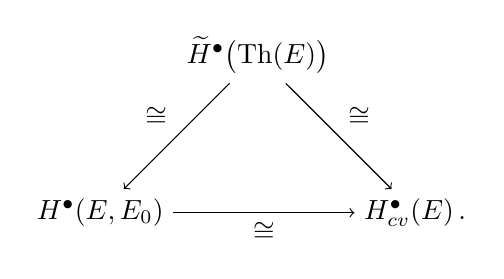
\begin{tikzpicture}[baseline=(current bounding box.east)]
                \node (TH) at (0, 0) {$\widetilde{H}^\bullet\bigl(\mathrm{Th}(E)\bigr)$};
                \node (R) at (-2, -2) {$H^\bullet(E,E_0)$};
                \node (CV) at (2, -2) {$H^\bullet_{\text{cv}}(E)\,.$};
                \draw[->] (TH) -- node[above left]{$\cong$} (R);
                \draw[->] (TH) -- node[above right]{$\cong$} (CV);
                \draw[->] (R) -- node[below]{$\cong$} (CV);
            \end{tikzpicture}
        \end{gather}
    \end{property}

    \newdef{\difficult{Thom spectrum}}{\index{spectrum!Thom}
        Let $E\rightarrow M$ be a vector bundle. The Thom spectrum of $E$ is defined as the suspension spectrum of its Thom space:
        \begin{gather}
            (\Sigma^\infty\mathrm{Th}(E))_n\cong\mathrm{Th}(\mathbb{R}^n\oplus E)\,,
        \end{gather}
        where $\mathrm{Th}(\mathbb{R}^n\oplus E)\cong\Sigma^n\mathrm{Th}(E)$ was used.

        Now, consider the sequence $\seq{\xi}$ of \textit{universal vector bundles}. For every $\xi_n$, define the $n^{\text{th}}$ component space as follows:
        \begin{gather}
            MO_n := \mathrm{Th}(\xi_n)\,.
        \end{gather}
        The Whitney sum $\xi_n\oplus\mathbb{R}$ can be obtained as a pullback of $\xi_{n+1}$. This map induces a morphism $\Sigma MO_n\rightarrow MO_{n+1}$, which gives the $n^{\text{th}}$ structure map of `the' Thom spectrum $MO$.\footnote{Note that the Thom spectrum as defined here is not an $\Omega$-spectrum (\cref{topology:spectrum}), it is merely a sequential spectrum (prespectrum).}
    }

    \newdef{Euler class}{\index{Euler!class}
        Consider a vector bundle $E\rightarrow M$ together with its Thom class $\Phi$. The Euler class $e(E)$ is defined as the pullback $s_0^*\Phi$ of the Thom class along the zero section of $E$.
    }
    \begin{property}
        If the orientation of $E$ is reversed, the Euler class changes sign.
    \end{property}
    The following property distinguishes the Euler class among all characteristic classes of $E$.
    \begin{property}[Normalization]
        If the vector bundle admits a nowhere-vanishing section, its Euler class vanishes.
    \end{property}

\subsection{\v{C}ech--de Rham complex}\label{section:cech_de_rham}

    \begin{theorem}[Mayer--Vietoris sequence]\index{Mayer--Vietoris!sequence}
        Consider a smooth manifold $M$ with an open covering $U\cup V$. The cohomology of $U,V$ is related to that of $M$ by the following short exact sequence:
        \begin{gather}
            0\longrightarrow H^\bullet(M)\overset{\iota_U\oplus\iota_V}{\longrightarrow} H^\bullet(U)\oplus H^\bullet(V)\overset{\pi_2-\pi_1}{\longrightarrow} H^\bullet(U\cap V)\longrightarrow 0\,.
        \end{gather}
    \end{theorem}

    \newdef{\v{C}ech--de Rham complex}{
        The \v{C}ech complex (\cref{sheaf:cech}) associated to the constant sheaf $\flat\mathbb{R}$, i.e.~the sheaf of locally constant functions.
    }

    The Mayer--Vietoris sequence can be generalized to a statement about the \v{C}ech-de Rham complex.
    \begin{property}[Mayer--Vietoris sequence]
        The horizontal complex
        \begin{gather}
            0\longrightarrow\Omega^\bullet(M)\longrightarrow\prod_{i_0}\Omega^\bullet(U_{i_0})\longrightarrow\prod_{i_0,i_1}\Omega^\bullet(U_{i_0i_1})\longrightarrow\cdots
        \end{gather}
        is acyclic, i.e.~the $\delta$-cohomology of the \v{C}ech--de Rham complex vanishes.
    \end{property}

    An important corollary is that one can compute the (de Rham) cohomology of $M$ using the above double complex.
    \begin{property}
        The restriction map $\Omega^\bullet(M)\rightarrow C^\bullet(\mathcal{U};\Omega^\bullet)$ induces an isomorphism in cohomology.
    \end{property}
    One can also augment the \v{C}ech--de Rham complex in the other direction by the kernel of the de Rham differential in degree 1. These are the locally constant functions on the intersections $U_{i_0\ldots i_p}$. The cohomology of this augmenting sequence $C^\bullet(\mathcal{U};\flat\mathbb{R})$ is called the \textbf{\v{C}ech cohomology} of $M$.\index{Cech!cohomology} By the same reason as for why the Mayer--Vietoris sequence implied the above theorem, the following theorem is obtained.
    \begin{theorem}[\v{C}ech $=$ de Rham]
        For a smooth manifold $M$, admitting a good cover $\mathcal{U}$, the \v{C}ech cohomology of $\mathcal{U}$ is isomorphic to the de Rham cohomology of $M$:
        \begin{gather}
            H^\bullet(M)\cong\check{H}^\bullet(\mathcal{U};\flat\mathbb{R})\,.
        \end{gather}
        By noting that good covers are \textit{cofinal} in the set of open covers, one can pass to the full \v{C}ech cohomology:
        \begin{gather}
            H^\bullet(M)\cong\check{H}^\bullet(M;\flat\mathbb{R})\,.
        \end{gather}
    \end{theorem}
    \begin{result}
        All compact manifolds admit a finite good cover and, hence, have finite-dimensional de Rham cohomology.
    \end{result}

    \begin{property}[Exponential sequence]
        Consider the following exact sequence of topological groups:
        \begin{gather}
            0\longrightarrow\mathbb{Z}\overset{2\pi}{\longrightarrow}\mathbb{C}\overset{\exp}{\longrightarrow}\mathrm{U}(1)\longrightarrow0\,.
        \end{gather}
        Let $(M,\mathcal{O}_M)$ be a \textit{complex manifold} (see \cref{chapter:complex_geometry}) or a smooth manifold and restrict the above sequence to the real numbers. The exact sequence induces an exact sequence of structure sheaves:
        \begin{gather}
            0\longrightarrow\flat\mathbb{Z}\longrightarrow\mathcal{O}_M\longrightarrow\mathcal{O}_M^\times\longrightarrow0\,.
        \end{gather}
        This, in turn, induces a long exact sequence in cohomology and, by \cref{sheaf:example_soft} (if $M$ is paracompact), the connecting homomorphism leads to an isomorphism:
        \begin{gather}
            \label{bundle:U1_cohomology_isomorphism}
            H^{\bullet+1}(M;\mathbb{Z})\cong\check{H}^\bullet\bigl(M;\mathrm{U}(1)\bigr)\,.
        \end{gather}
        Note that the cohomology on the right-hand side is not singular cohomology. Singular $\mathrm{U}(1)$-valued cohomology could also be related to integral cohomology through the \textit{universal coefficient theorem}, but extra terms involving Ext-functors would appear.
    \end{property}

\subsection{Nonorientable manifolds}

    This section gives a differential-geometric incarnation of \cref{section:local_coefficients} on local coefficients.

    \newdef{Twisted cohomology}{\index{cohomology!twisted}
        Let $E\rightarrow M$ be a flat vector bundle over $M$. By \cref{bundle:twisted_differential}, the algebra $\Omega^\bullet(M)\otimes E$ can be given the structure of a differential graded algebra (\cref{homalg:dg_algebra}) and, hence, gives rise to a cohomology theory $H^\bullet(M;E)$. This is called the $E$-twisted de Rham cohomology of $M$.
    }
    \begin{remark}
        According to the remark following \cref{bundle:twisted_differential}, attention should be payed to which trivialization was used in the construction of $H^\bullet(M;E)$. However, it can be shown that two trivializations give rise to the same $E$-twisted cohomology if they admit a common refinement for which the induced sections differ by a locally constant matrix in $\GL(n,\mathbb{R})$.
    \end{remark}

    If one takes $E=o(M)$ to be the orientation line bundle over $M$, the (honest) densities of \cref{bundle:honest_density} are obtained. The cohomology of this complex is simply called the \textbf{twisted de Rham cohomology}.
    \begin{property}[Isomorphism]
        The twisted cohomologies defined by two trivializations induced from atlases on $M$ are isomorphic.\footnote{Although one almost always works with a natural trivialization, i.e.~the open subsets of $M$ are obtained from charts on $M$, this is technically not necessary. For more `exotic' cases, the isomorphisms not always exist.}
    \end{property}
    \begin{property}[Trivial twisting]
        If $M$ is orientable, its twisted cohomology is isomorphic to its ordinary (de Rham) cohomology. More generally, the $E$-twisted de Rham cohomology is isomorphic to the ordinary de Rham cohomology whenever $E$ is trivial.
    \end{property}

    Poincar\'e duality (\cref{bundle:poincare_duality}) can be generalized almost verbatim to the twisted case.
    \begin{theorem}[Poincar\'e duality]\index{Poincar\'e!duality}
        Integration of densities induces the following isomorphism:
        \begin{gather}
            H^k(M)\cong\left(H^{m-k}_c\bigl(M;o(M)\bigr)\right)^*\,.
        \end{gather}
        If $M$ is of finite type, the converse also holds:
        \begin{gather}
            H^k_c(M)\cong\left(H^{m-k}\bigl(M;o(M)\bigr)\right)^*\,.
        \end{gather}
    \end{theorem}
    The Thom isomorphism also holds for nonorientable bundles.
    \begin{theorem}[Thom isomorphism]\index{Thom!isomorphism}
        Let $E\rightarrow M$ be a rank-$n$ vector bundle. Fibre integration gives the following isomorphism:
        \begin{gather}
            H^{\bullet+n}_{\text{cv}}(E)\cong H^\bullet\bigl(M;o(E)\bigr)\,.
        \end{gather}
    \end{theorem}

\subsection{\difficult{Generalized cohomology}}

    In this section, some statements from singular/de Rham cohomology on vector bundles are generalized to statements about the generalized (Eilenberg--Steenrod) cohomology theories from \cref{section:eilenberg_steenrod}. In the remainder of this section, $E^\bullet$ will denote a multiplicative generalized cohomology theory.\footnote{`Multiplicative' indicates that there exists a cup product such that every group $E^\bullet(M)$ becomes a graded ring.}

    \newdef{Orientation}{\index{orientation}\index{Thom!class}
        Consider a rank-$n$ vector bundle with typical fibre $V$. An $E$-orientation or $E$-\textbf{Thom class} is a cohomology class $u\in\widetilde{E}^n(\mathrm{Th}(V))$ that restricts to a generator on every fibre of $V$.
    }

    \todo{COMPLETE}

\section{Morse theory}\label{section:morse}
\subsection{Morse functions}

    \newdef{Nondegeneracy}{\index{critical!point}\index{nondegeneracy}\label{manifold:nondegeneracy}
        At a critical point $p\in M$, the Hessian of a smooth function $f:M\rightarrow\mathbb{R}$, in local coordinates, gives a well-defined quadratic form. A critical point is said to be nondegenerate if the Hessian is nonsingular there.
    }

    \newdef{Morse function}{\index{Morse!function}\label{manifold:morse_function}
        Let $M$ be a smooth manifold. A smooth function is called a Morse function if it has no degenerate critical points.
    }

    \begin{property}[Density]
        The set of Morse functions is open and dense in the $C^2$-topology (see \cref{section:jet_bundles} on \textit{jet spaces}).
    \end{property}

    \newdef{Palais--Smale condition}{\index{Palais--Smale condition}
        A smooth function $f\in C^1(M)$ is said to satisfy the Palais--Smale condition if every sequence $\seq{x}\subset M$ with
        \begin{enumerate}
            \item $|f(x_n)|$ bounded for all $n\in\mathbb{N}$, and
            \item $\|Df(x_n)\|\longrightarrow0$
        \end{enumerate}
        contains a convergent subsequence. It is clear that every smooth function on a compact manifold and every proper function (\cref{topology:proper_function}) satisfies this condition.
    }
    \begin{result}
        If $f\in C^1(M)$ is Morse and satisfies the Palais--Smale condition, it has only finitely many critical points in every bounded subset or in any set where $f$ is bounded.
    \end{result}

    \newdef{Morse index}{\index{index}
        Consider a Morse function $f\in C^\infty(M)$. The number of negative eigenvalues at a critical point $p\in M$ is called the (Morse) index of $f$ at $p$. This is often denoted by $\lambda_p(f)$.

        To any Morse function one can associate a series called the \textbf{Morse counting-series}:
        \begin{gather}
            M_t(f) := \sum_{p\in\mathrm{crit}(f)}t^{\lambda_p(f)}\,.
        \end{gather}
        If $M$ is compact, the nondegeneracy condition implies that the above sum only has a finite number of terms.
    }

    \begin{property}[Morse lemma]\index{Morse!lemma}
        Consider a Morse function $f:M\rightarrow\mathbb{R}$ and let $p\in M$ be a nondegenerate critical point of $f$. There exists a chart $(U,x_1,\ldots,x_n)$ around $p$ such that $x_i(p)=0$ and
        \begin{gather}
            f|_U(x) = f(p) - x_1^2-\cdots + x_k^2+\cdots\,,
        \end{gather}
        where $k=\lambda_p(f)$ is the Morse index of $f$.
    \end{property}
    \begin{result}
        The critical points of a Morse function are isolated.
    \end{result}
    \begin{remark}[Morse--Palais lemma]\index{Morse--Palais}
        The Morse lemma can be generalized to open subsets of Banach spaces (and thus to infinite-dimensional manifolds).
    \end{remark}

    \newdef{Self-indexing function}{
        A Morse function whose value at every critical points is equal to its index.
    }

    \todo{COMPLETE}

\subsection{Morse--Bott functions}

    By the Morse lemma, the critical points of a Morse function are isolated. When this condition is relaxed, a more general class of functions is obtained. Here, it is assumed that $M$ comes equipped with a covariant derivative (\cref{section:linear_connections}).

    \newdef{Morse--Bott function}{\index{Morse--Bott function}
        A smooth function $f:M\rightarrow\mathbb{R}$ for which the critical set $\mathrm{Crit}(f)$ is a submanifold of $M$ and at every point $p\in\mathrm{Crit}(f)$ the tangent space is the kernel of the Hessian of $f$, i.e.~its Hessian is nondegenerate in the normal directions at every critical point.
    }

\subsection{Morse homology}\label{section:morse_homology}

    \newdef{Gradientlike vector field}{\index{vector field!gradientlike}
        Consider a Morse function $f\in C^\infty(M)$. A vector field $X$ is said to be gradientlike with respect to $f$ if is satisfies the following conditions:
        \begin{enumerate}
            \item For all $p\not\in\mathrm{Crit}(f):X|_p(f)>0$.
            \item For all $p\in\mathrm{Crit}(f)$, there exists a Morse chart containing $p$ such that
            \begin{gather}
                X = -2\sum_{i=1}^{\lambda_p(f)}x^i\partial_i+2\sum_{i=\lambda_p(f)+1}^{\dim(M)}x^i\partial_i\,.
            \end{gather}

        \end{enumerate}
        Its flow lines have the same orientation away from critical points and it coincides with the gradient at critical points. Furthermore, such vector fields always exist.
    }
    \begin{property}
        Let $f\in C^\infty(M)$ be a Morse function on a compact\footnote{This property also holds more generally, but then one has to restrict to integral curves $\gamma$ whose image $f(\gamma)$ is bounded.} manifold and consider a gradientlike vector field $X$ with respect to $f$. The integral curves of $X$ are complete and the limits are critical points of $f$.

    \end{property}

    \newdef{Stable and unstable manifold}{\index{stable!manifold}
        Let $f\in C^\infty(M)$ be a Morse function and consider a gradientlike vector field $X$ (with respect to $f$). For every critical point $p$ of $f$, the stable and unstable manifold of $X$ are defined as follows:
        \begin{gather}
            W^\pm_p(X) := \bigl\{x\in M\bigm\vert\lim_{t\rightarrow\pm\infty}\Phi_t(x)=p\bigr\}\,,
        \end{gather}
        where $\Phi_t$ denotes the flow of $-X$. These sets carry the structure of smooth manifolds that are locally diffeomorphic to $\mathbb{R}^{\dim(M)-\lambda_p(f)}$ and $\mathbb{R}^{\lambda_p(f)}$, respectively.
    }

    \newdef{Morse--Smale pair}{\index{Morse--Smale pair}
        Let $f\in C^\infty(M)$ be a Morse function and consider a gradientlike vector field $X$ with respect to $f$. If, for all critical points $p,q\in\mathrm{Crit}(f)$, one has that
        \begin{gather}
            W^+_p(X)\pitchfork W^-_q(X)\,,
        \end{gather}
        the pair $(f,X)$ is called a Morse--Smale pair.
    }
    \begin{property}
        If $M$ is compact, there exists a self-indexing Morse--Smale pair.
    \end{property}

    \begin{property}
        For every Morse function on a compact manifold, there exists a generic metric such that $(f,\nabla f)$ is Morse--Smale.
    \end{property}

    From here on, it will be assumed that, given a Morse function $f\in C^\infty(M)$, the pair $(f,\nabla f)$ is Morse--Smale. Let $\mathcal{M}(p,q)$ denote the set of integral curves of $-\nabla f$ that start at $p$ and end at $q$, i.e.~the integral curves $\gamma$ that satisfy
    \begin{gather}
        \gamma([0,1])\subset W^-_p(\nabla f)\cap W^+_q(\nabla f)\,.
    \end{gather}
    By the structure of the stable and unstable manifolds, this solution space has dimension $\lambda_p(f)-\lambda_q(f)$. Integral curves can be arbitrarily reparametrized. To obtain a well-defined moduli space $\overline{\mathcal{M}}(p,q)$, this $\mathbb{R}$-action is quotiented out (it is free and proper, so the resulting space is again a smooth manifold).

    \newdef{Morse homology}{\index{Morse|seealso{homology}}\index{homology!Morse}
        The chain groups are defined as follows
        \begin{gather}
            CM_k(M,f) := \bigoplus_{\substack{p\in\mathrm{Crit}(f)\\\lambda_p(f)=k}}\mathbb{Z}\langle p \rangle\,.
        \end{gather}
        For critical points $p,q\in\mathrm{Crit}(f)$ such that $\lambda_p(f)=\lambda_q(f)+1$, the moduli space is a discrete, compact set. This allows to define the boundary operator as follows:
        \begin{gather}
            \partial p := \sum_{\substack{q\in\mathrm{Crit}(f)\\\lambda_q(f)=\lambda_p(f)-1}}\left|\,\overline{\mathcal{M}}(p,q)\right|\langle q \rangle\,.
        \end{gather}
        One can show that $\partial^2=0$. Morse homology is defined as the homology of this complex:
        \begin{gather}
            HM_\bullet(M,f) := \frac{\ker(\partial)}{\im(\partial)}\,.
        \end{gather}
    }

\section{Differential operators}

    In this section, the study of PDEs is generalized to vector bundles. The case of PDEs on $\mathbb{R}^n$ was treated in \cref{chapter:pde}.

    \newdef{Differential operator}{\index{differential!operator}\index{elliptic!operator}\label{bundle:differential_operator}
        A (linear) differential operators between two vector bundels $E,F$ over the same base manifold $M$ is a linear map $D:\Gamma(E)\rightarrow\Gamma(F)$ that can locally be expressed as a system of partial differential equations. The principal symbols on different charts glue together to give a globally defined morphism
        \begin{gather}
            \sigma_D:T^*M\rightarrow\hom(\pi^*E,\pi^*F)\,,
        \end{gather}
        where $\pi:T^*M\rightarrow M$ is the cotangent bundle projection.

        By extension of the ordinary theory of PDEs, one says that the differential operator is \textbf{elliptic} (hyperbolic, ...) if its associated PDE is elliptic (hyperbolic, ...). E.g.~a differential operator is said to be hyperbolic if the the above morphism is invertible for all cotangent vectors.
    }

    \newdef{Normally hyperbolic operators}{\index{hyper-!bolic operator}
        Consider a \textit{(pseudo)Riemannian} vector bundle $E$ (see \cref{chapter:riemann}). A linear differential operator on $E$ is said to be normally hyperbolic if its principal symbol is proportional to the given metric.
    }

\subsection{Elliptic complexes}

    \newdef{Elliptic complex}{\index{elliptic!complex}
        Consider a collection of vector bundles $\{\pi_n:E_n\rightarrow M\}_{n\in\mathbb{N}}$ together with a sequence of differential operators $\bigl(D_n:C^\infty(E_n)\rightarrow C^\infty(E_{n+1})\bigr)_{n\in\mathbb{N}}$. This system is called an elliptic complex if it is a cochain complex, i.e.~$D_{n+1}\circ D_n = 0$, and if the induced sequence $\bigl(\sigma_p(\xi)(D_n)\bigr)_{n\in\mathbb{N}}$ is exact for all $x\in M$ and $\xi\neq0$.
    }

    \todo{COMPLETE}